%\fancyhead[RO,LE]{\thepage}
%\fancyfoot{}

\chapter{Anti-unification of Logged Java Classes} \label{ch4} \label{methodology}
In Chapter~\ref{background} we provided background information on higher-order anti-unification modulo theories---a theoretical framework for constructing a generalization from two given structures---and we described how the Jigsaw tool applies this framework on AST structures of two given Java classes to determine potential structural correspondences between them. We now consider how these frameworks could help us (1)~to generalize ASTs of two Java classes containing logging calls and (2)~to develop a similarity measure with a focus on logging calls that can provide us with useful information for clustering LJCs in a later phase.

Recall the general point of this study: we aim to provide a concise description of where logging calls happen in the source code through constructing structural generalizations that represent the detailed structural similarities and differences of LJCs. To this end, we should develop an algorithm that:
\begin{itemize} [leftmargin=.3in]
\item classifies LJCs into groups using a measure of similarity such that entities in each group has maximum similarity with each other and minimum similarity to other ones
\item abstracts structural correspondences of LJCs of each group into a structural generalization representing the similarities and differences
\end{itemize}
%A generalization mechanism could be used to abstract commonalities in several structures containing logging calls into a more general structure; 
%The higher-order anti-unification modulo theories framework could assist us in constructing a structural generalization from a pair of LCSs. Also, A modified version of a hierarchical clustering suited for our application could assist us to construct a generalization from a set of LJCs.

%To construct a structural generalization from a pair of LJCs, we developed a prototype tool that applies the Jigsaw framework to find candidate correspondences between two ASTs and uses higher-order anti-unification modulo theories to generalize the structures. It takes the source code of two logged Java classes as input and performs a sequence of six actions on them, outlined by the algorithm \func{Anti-Unification}: (1) we input into the algorithm the ASTs of two given logged Java classes, constructed via the Eclipse Java Development Tools (JDT) framework; (2) we generate an augmented form of AST (called a CAST) using the Jigsaw framework, where each node holds a list of candidate correspondence connections between the two ASTs (line~1) (see Section~\ref{meth-CAST}); (3) we extend the CAST structure to a higher-order extended structure (called an AUAST) and apply some constraints to prevent the anti-unification of logging calls with anything else (lines~2--3) (see Sections~\ref{meth-constructAUAST} and~\ref{meth-constraints}); (4) we determine the best correspondence for each node of the AUASTs with the highest similarity and we remove the other correspondence connections involving the nodes (line~4) (see Section~\ref{meth-correspondence}); (5) we anti-unify structural properties with their best correspondence to construct an approximation of the best anti-unifier to our problem with a special attention to logging calls (line~5) (see Section~\ref{meth-antiUnifier}); and (6) we measure similarity (line~6) (see Section~\ref{meth-similarity}).

To construct structural generalizations from a set of LJCs, we developed a prototype tool that applies the Jigsaw framework to find candidate correspondences between two ASTs, the HOAUMT to generalize the structures, and a modified version of the agglomerative hierarchical clustering algorithm to classify a set of LJCs using a measure of similarity. As explained in Section~\ref{AUAST}, the AST structure should be extended to AUAST structure that allows the insertion of variables in place of any node, which is required for HOAUMT. 


Our hierarchical clustering algorithm is a bottom-up approach that starts with singleton clusters, where each contains one AUAST. In every iteration, it merges the closest clusters which are the clusters with maximum similarity between their AUASTs. Therefore, we need to develop a measure of similarity between each pair of AUAST and then construct an anti-unifier when it is needed to merge two clusters. 

The structural similarity between two given AUASTs is defined as the number of identical simple property values over total number of simple property values of the anti-unifier (see Section~\ref{meth-similarity}). To do so, we determine the best correspondences for each node and compute the structural matches between them. Our tool performs a sequence of 3 actions to determine the best correspondences between two AUASTs, outlined by the algorithm \func{Determine-Best-Correspondences}: (1) it generates all possible candidate correspondence connections between ASTs of two AUASTs using the Jigsaw framework (line~1) (see Section~\ref{meth-CAST}); (2) it applies some constraints to prevent the anti-unification of logging calls with anything else (line~2) (see Section ~\ref{meth-constraints}); (3) it determines the best correspondence for each node of AUASTs with the highest similarity and then removes the other correspondence connections involving those nodes (line~3) (see Section~\ref{meth-correspondence}); 

To construct an approximation of the best anti-unifier to our problem with a special attention to logging calls, a further step should be taken, which is anti-unification of each AUAST node with its best correspondence determined in the previous step through anti-unifying their structural properties (see Section~\ref{meth-antiUnifier}). Figure~\ref{fig:meth_overview} shows an overview of the general process of our anti-unification technique, as will be described in the following sections.


\begin{algorithm}
\caption{\func{Determine-Best-Correspondences}(\vars{auastA},\vars{auastB}) determines best correspondences between the two AUAST nodes \vars{auastA} and \vars{auastB}}
\label{overview}
\begin{algorithmic}[1]
\DetermineBest
   \State  $\func{Jigsaw-Correspondence}(\vars{auastA},\vars{auastB})$  
   \State $\func{Apply-Constrains}(\vars{auastA},\vars{auastB})$
   \State $ \func{Determine-Correspondences}(\vars{auastA})$
\end{algorithmic}
\end{algorithm}


%\begin{algorithm}
%\caption{Input into \func{Anti-unification}(\vars{auastA},\vars{auastB}) are AUAST nodes of two Java classes containing logging calls; this algorithm construct an anti-unified AUAST node through anti-unification of input node's structural properties} %and compute similarity between them with a focus on logging calls}
%\label{overview}
%\begin{algorithmic}[1]
%\Anti-unification
%    \State  $\func{Jigsaw-Correspondence}(\vars{auastA},\vars{auastB})$  
%   \State $\vars{auastA}, \vars{auastB} \gets \func{Apply-Constrains}(\vars{auastA},\vars{auastB})$
%   \State $\vars{list}  \gets \func{Determine-Best-Correspondences}(\vars{auastA})$
%     \State $\vars{compute-similarity} \gets \func{Compute-Similarity}(\vars{auastA},\vars{auastB})$
%    \State $\vars{anti-unifier} \gets \func{Anti-unify}(\vars{auastA},\vars{auastB})$
%\end{algorithmic}
%\end{algorithm}




\begin{figure} [H]
  \centering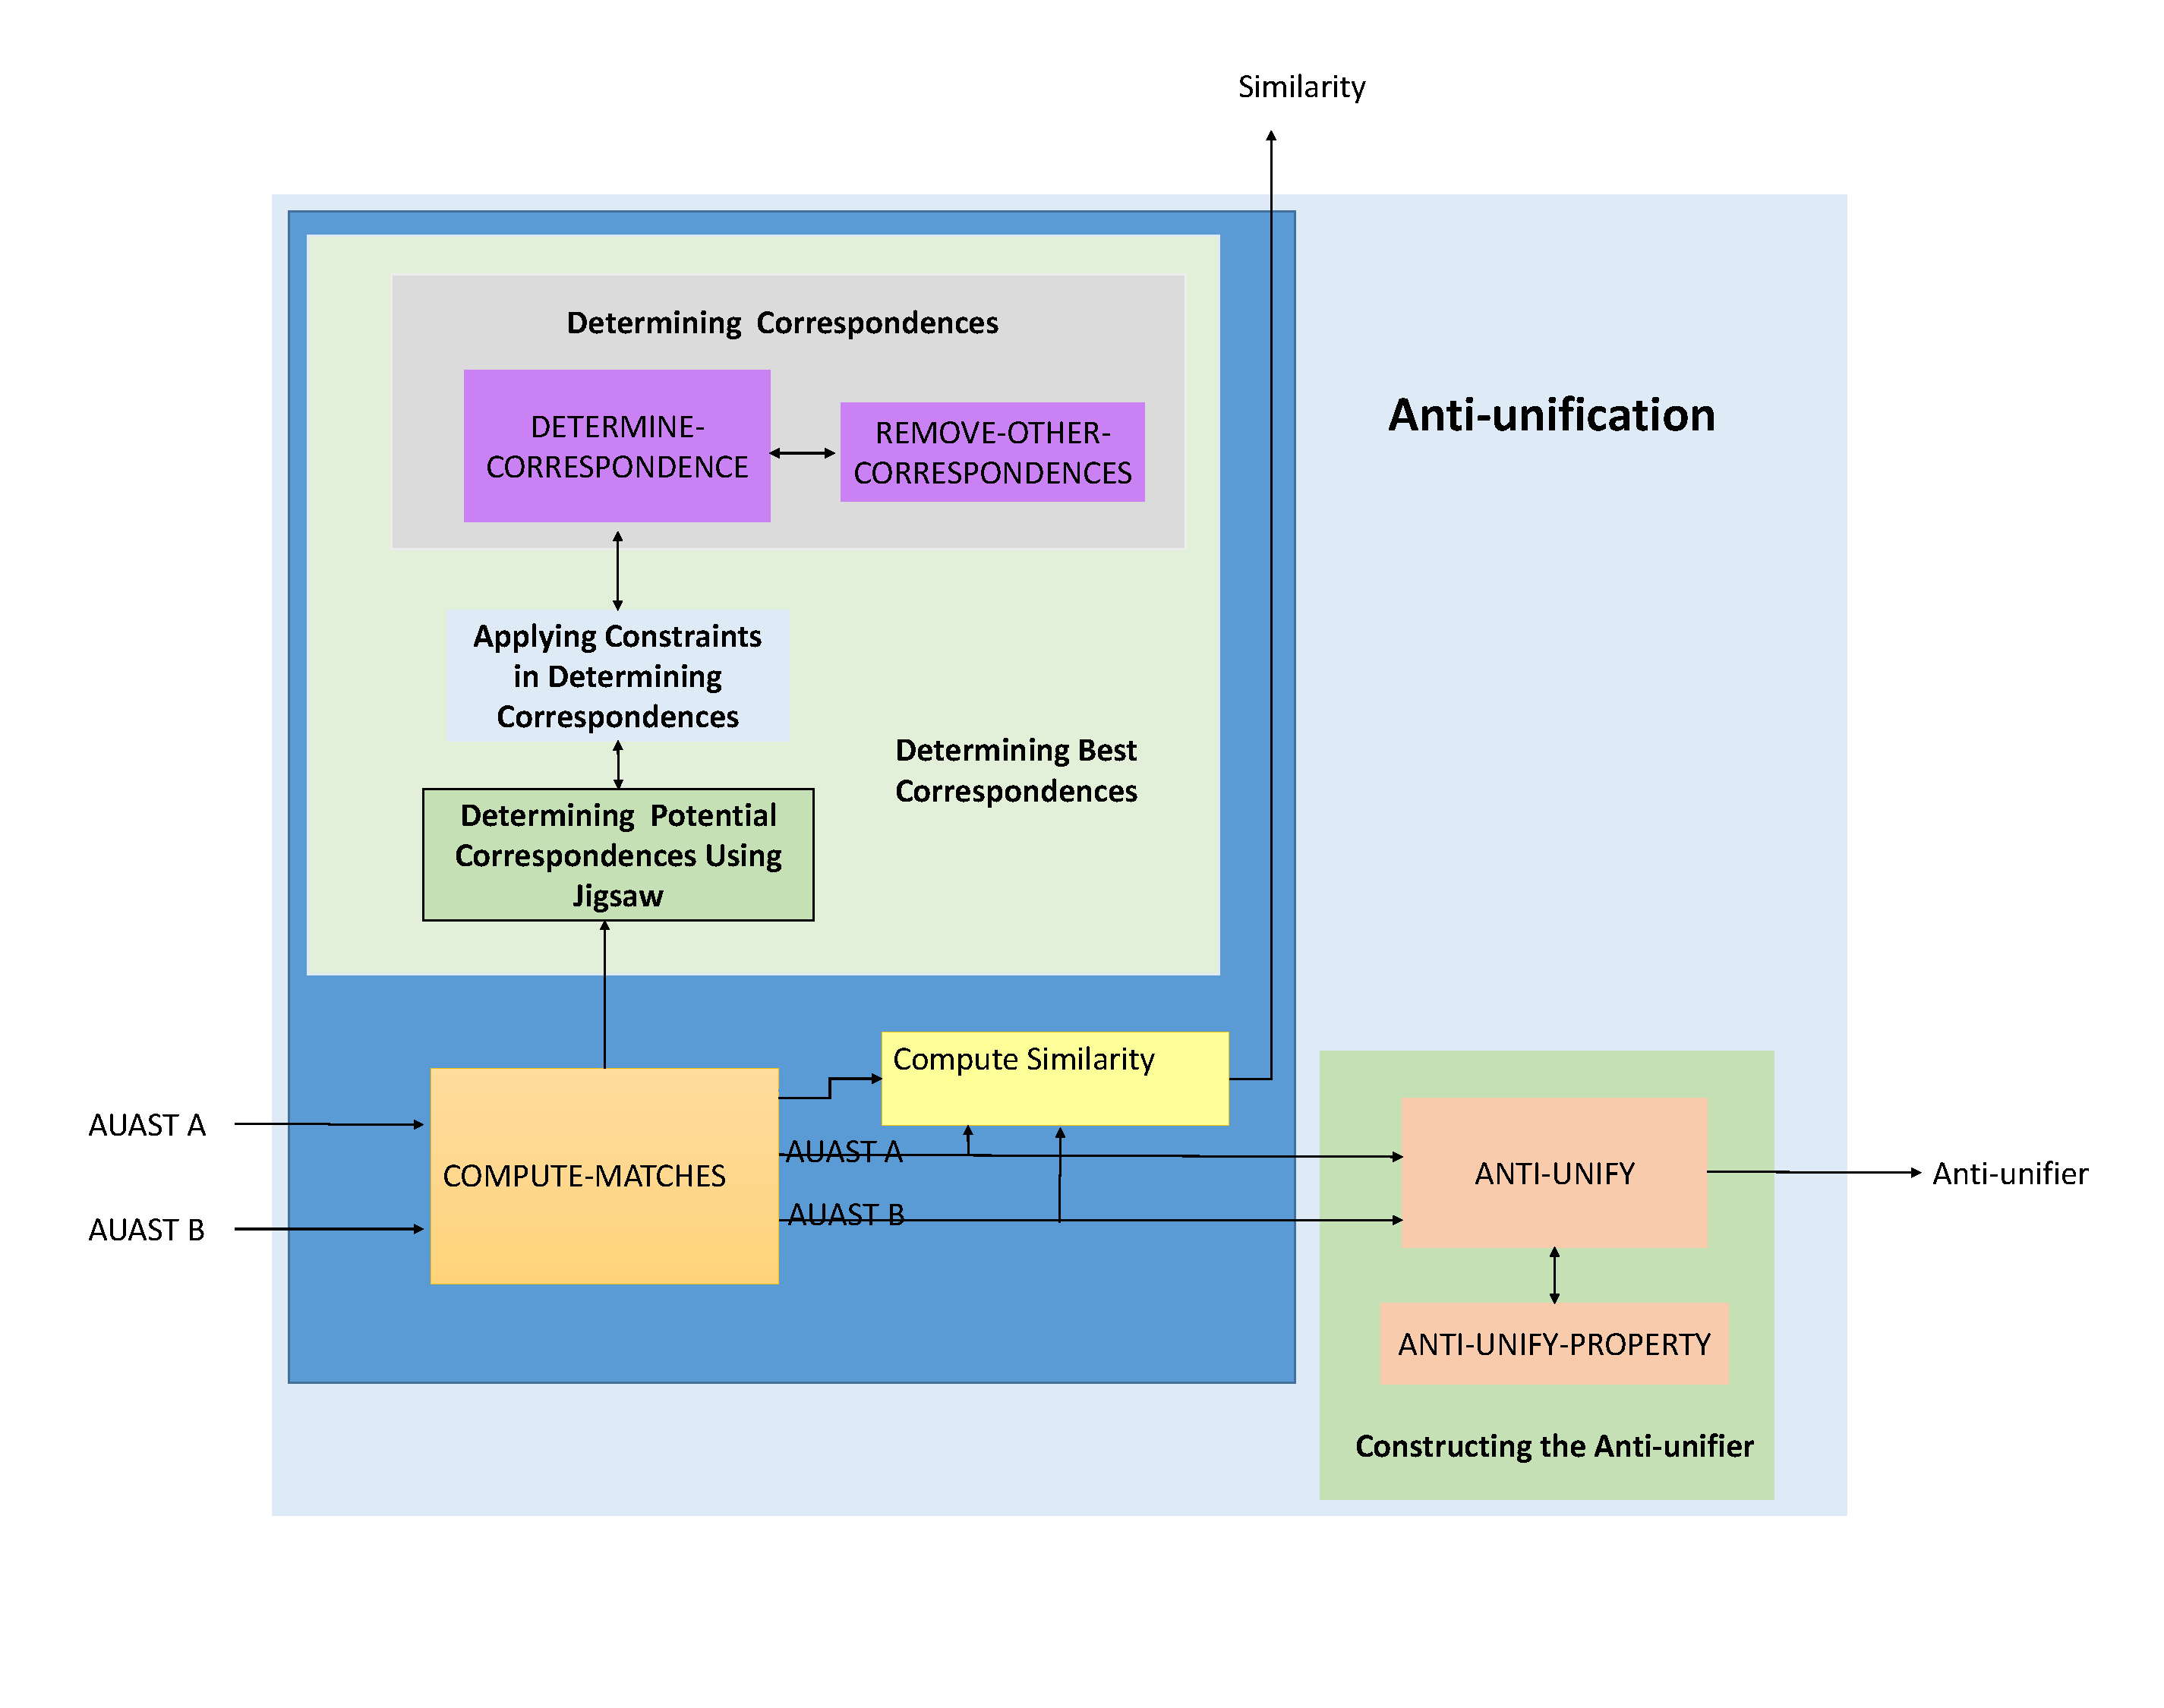
\includegraphics [width = \textwidth]{Drawing4/overview1.pdf}
  \caption{Overview of the system.}
  \label{fig:meth_overview}
\end{figure}


\section{Constructing the AUAST} \label{meth-constructAUAST}
The goal of this phase is to construct an extension of the AST structure that would allow the creation of an anti-unified structure. 
As described in Section~\ref{ch3-AU}, an anti-unified structure utilizes variables that must be substituted with a proper substructure to gain back to each original structure; however, the AST structure does not contain any variables thus an extended form of it is required, named AUAST, to address these limitation by allowing the insertion of variables in place of any node in the tree structure, including both subtrees and leaves, to indicate variations between original structures. the AUAST structure addresses the limitations of AST to construct an anti-unifier by adding the following structural properties:

\begin{itemize} [leftmargin=.4in]
\item \bold{Simple Variable Property}: an extension of simple property referring to two simple property values to allow the insertion of variables in place of leaves.
\end{itemize}
\begin{itemize} [leftmargin=.4in]
\item \bold{Child Variable Property}: an extension of child property referring to two child nodes to allow the insertion of variables in place of subtrees.

\end{itemize}

We provide an example to demonstrate the AUAST structure, which is limited to log method invocation subtrees of the sample Java classes shown in Figure~\ref{fig:constructAUast}. The log method invocation nodes both contains \texttt{EXPRESSION}, \texttt{ARGUEMENTS}, and \texttt{NAME} structural properties which are made up of \texttt{\bold{Log}}, \texttt{\bold{Log}}, \texttt{\bold{WARNING}} simple values for the AUAST1 and  \texttt{\bold{Log}}, \texttt{\bold{Log}}, \texttt{\bold{ERROR}} simple values for the AUAST2, respectively. The structural representation of the AUASTs as defined in Section~\ref{back-str} is \texttt{EXPRESSION[EXPRESSION[IDENTIFIER[\bold{Log}]], ARGUMENTS[QUALIFIER[IDENT\\IFIER[\bold{Log}]], NAME[IDENTIFIER[\bold{WARNING}]]}
for the AUAST1 and \texttt{EXPRESSION[EX\\PRESSION[IDENTIFIER[\bold{Log}]], ARGUMENTS[QUALIFIER[IDENTIFIER[\bold{Log}]], \\NAME[IDENTIFIER[\bold{ERROR}]]}
for the AUAST2, where the words capitalized represents subtrees and the words shown in bold represents leaves of the tree structure.


\begin{figure} [H]
  \centering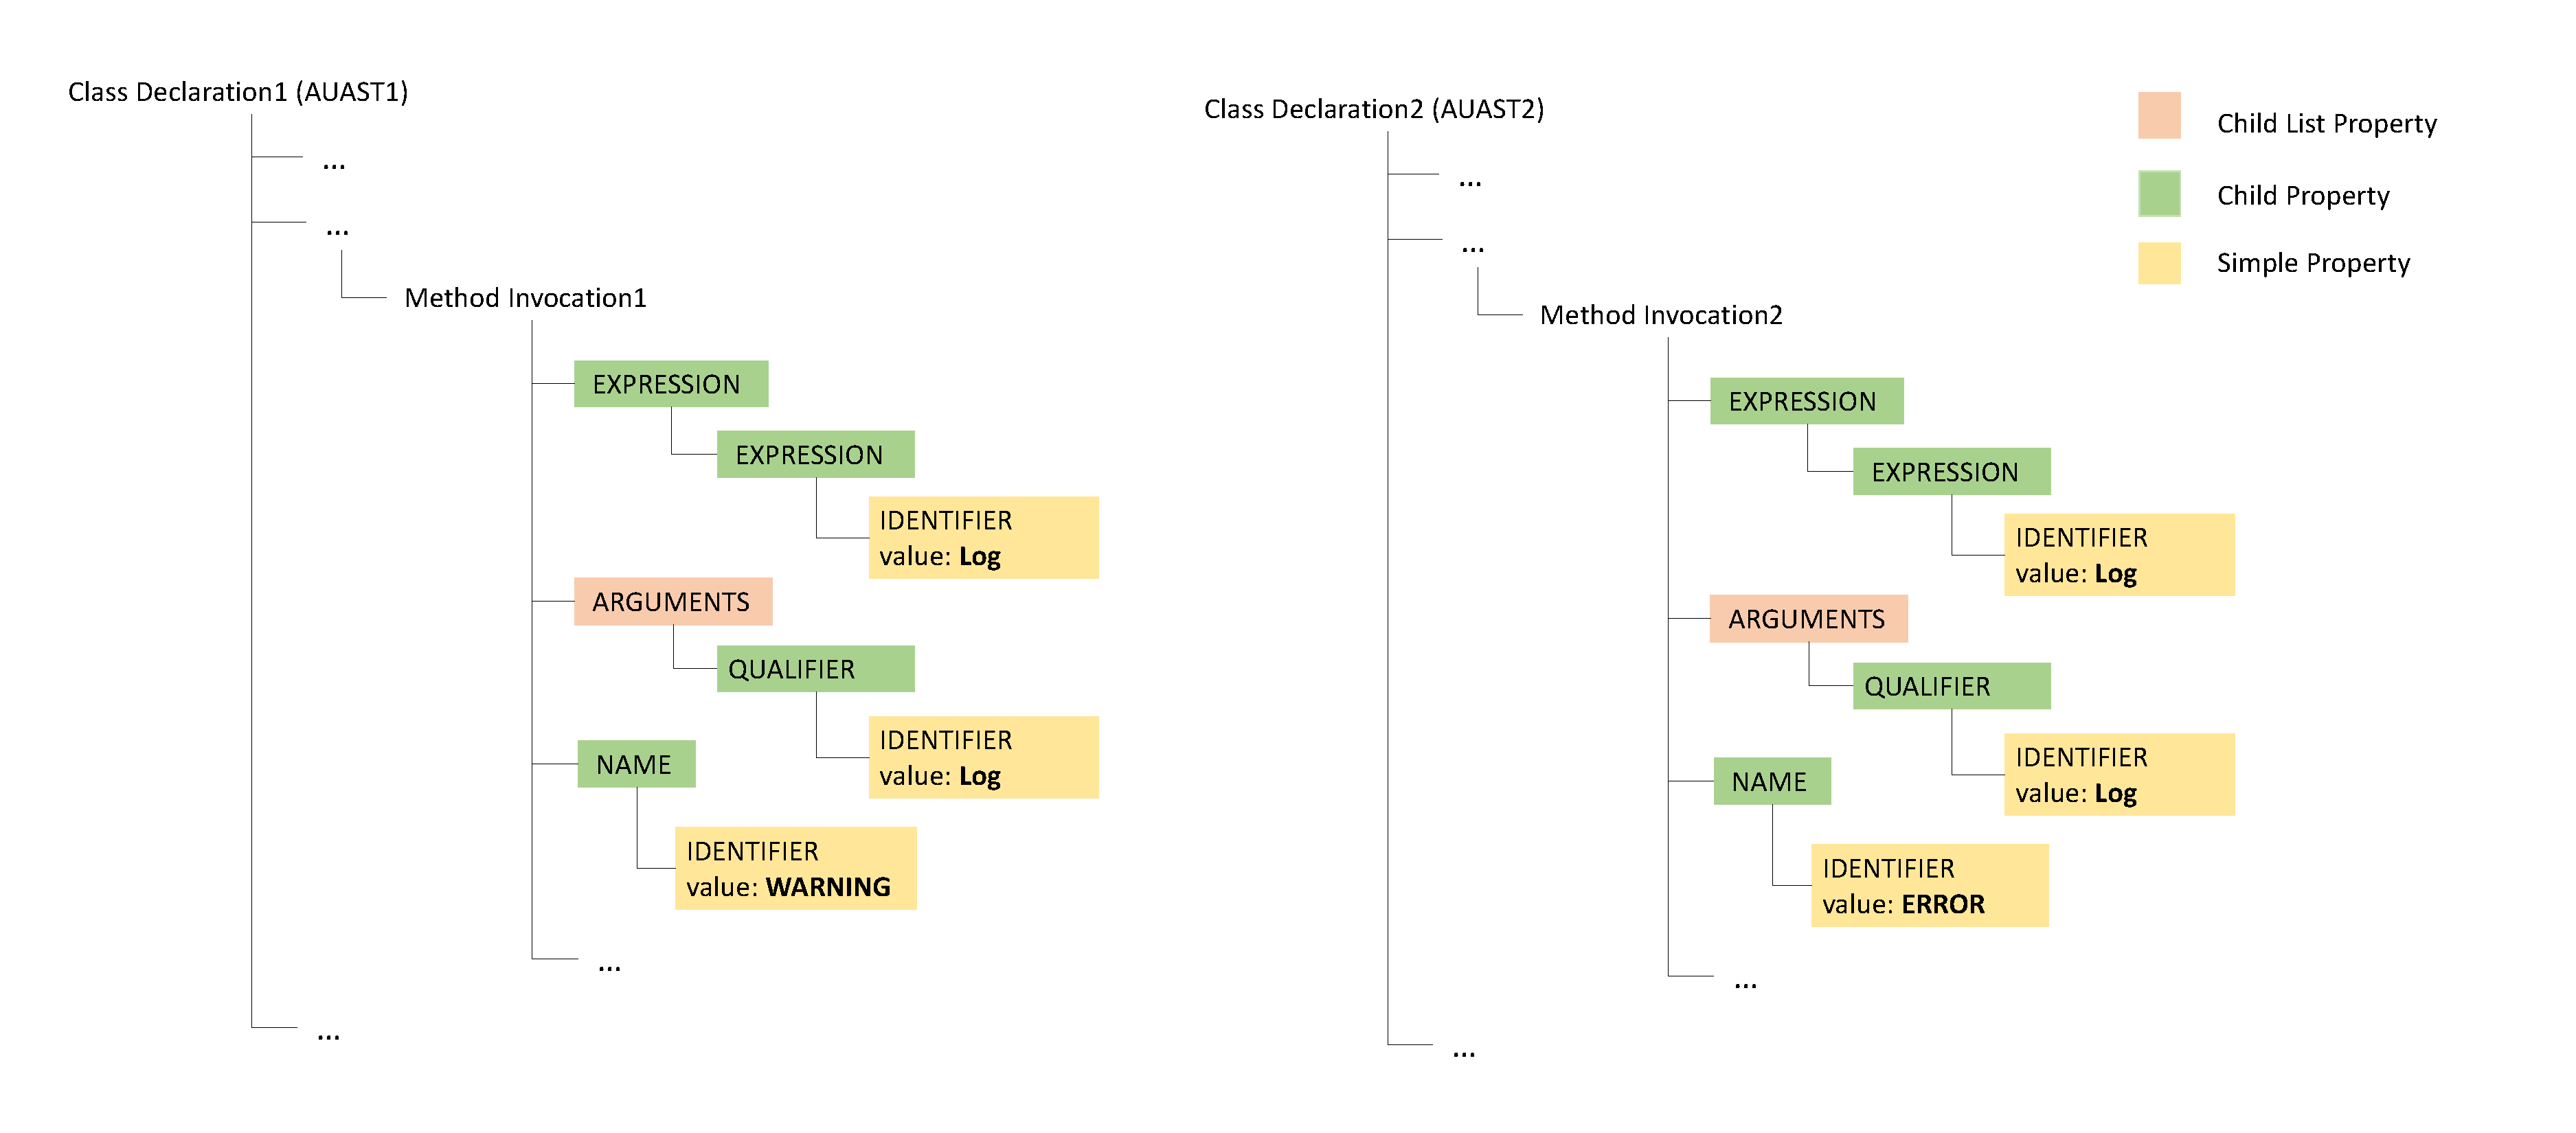
\includegraphics [width = \textwidth, height = 0.4\textheight]
  {Drawing4/structure1.pdf}
  \caption{The AUASTs of log Method Invocation nodes from the Java classes in Figure~\ref{ch3-ex1} and Figure~\ref{ch3-ex2}.}
  \label{fig:constructAUast}
\end{figure}


\section{Deteremining Correspondences Using Jigsaw} \label{meth-CAST}
% I should write its explanation
 
\begin{algorithm}
\caption{\func{Jigsaw-Correspondence}(\vars{auastA},\vars{auastB}) determines all the potential correspondences between nodes of two given AUASTs}
\label{overview}
\begin{algorithmic}[1]
\JigsawCorr
\For {$\vars{astA} \in  \vars{auastA}$}	
\For {$\vars{astB} \in  \vars{auastB}$}		
	\State  $\vars{castA},\vars{castB} \gets \func{Jigsaw-Anti-unify}(\vars{astA},\vars{astB})$
\EndFor	
\EndFor    
\end{algorithmic}
\end{algorithm}




\section{Constraints in Determining Correspondences}  \label{meth-constraints}
To construct an anti-unifier of two AUASTs with a focus on logging calls, some constraints should be applied prior to determining the best correspondences. The first constraint (as described below) should be applied to prevent the anti-unification of log method invocation nodes with any other type of node.
\begin{constraint}
A logging call should either be anti-unified with another logging call or should be anti-unified with \nothing.
\end{constraint}	
	
This constraint creates a further constraint, which is:

\begin{constraint}
A structure containing a logging call should be anti-unified with a corresponding structure containing another logging call or should be anti-unified with \nothing.
\end{constraint}


To provide an example to illustrate it consider ATSs of two Java classes in Figure~\ref{fig:meth-ast-1}. Jigsaw creates a correspondence connection between the two log method invocation nodes and the two \code{if} statements. As is clear, the second \code{if} statement contains a logging call, while there is no corresponding logging call in the first one. According to the first constraint, two log method invocation nodes should be anti-unified together. On the other hand, a correspondence connection is created between the two \code{if} statements; however, anti-unification of these statements includes anti-unifying their children nodes as well. Thus, statements inside the body of \code{if} statements must be anti-unified with each other, indicating that log method invocation inside the body of \code{if} statement in the second example should be anti-unified with \nothing, which is contrary to our first assumption. In order to comply with the first constraint, the correspondence connection between two \code{if} statements should be deleted, leading us to apply the second constraint.

Our approach applies these constraints by taking the following steps prior to determining correspondences:
\begin{enumerate} [leftmargin=.4in]
\item	Augment a property to AUAST node to mark log method invocation nodes and structures enclosing them as ``logged''.

\item	Remove correspondence connections where one node is marked as ``logged'' and the corresponding node is not.
\end{enumerate}


\section{Determining Correspondences} \label{meth-correspondence}
As explained in Section~\ref{meth-CAST}, each node of the AUAST structure holds a list of candidate correspondence connections where each represents an anti-unifier. Despite having multiple potential anti-unifiers, we need to determine one single anti-unifier that is helpful to solve our problem. In general, higher order anti-unification modulo theories is undecidable [Cottrell et al., 2008]. That is, the complexity of determining the most optimal MSA is undecidable, but our desire is to create one of the best MSAs to approximate the optimal one that can sufficiently solve our problem, thus the anti-unification process should construct an anti-unifier that is the best approximate fit for our application. To this end, a greedy selection algorithm has been used, which is an approximation technique to determine the best correspondence for each node in the AUAST so constructing the anti-unifier that is approximately the best fit to our problem. As a result, each node can either be anti-unified with its best correspondence in the other AUAST or with \nothing.

\func{Determine-Correspondence} algorithm greedily selects the most similar correspondence as the best fit for each node in AUAST. It takes one of the AUASTs, visiting the AUAST nodes therein to store all candidate correspondence connections between the two AUAST nodes in a list, which is sorted in a descending order based on the Jigsaw similarity measure (lines~1--8). The correspondence connection with the highest similarity value is determined as the best fit for the two nodes involved (lines~9--11); all other correspondence connections involving these two nodes are removed using \func{Remove-Other-Correspondences} algorithm (line~10). This process terminates when no more correspondence connections is left in the list.
\begin{algorithm}
\caption{\func{Determine-Correspondence}(\vars{auastA}) takes in an AUAST node and create a list of correspondence connections containing the best correspondence to each node in the AUAST.}
\label{alg-determine}
\begin{algorithmic}[1]
\CreateList
    \State $\vars{list} \gets \func{()}$
    \State $\vars{nodes} \gets \func{visitor}(\vars{auastA})$
	  \For {$\vars{node} \in \vars{nodes}$}
	
				\For {$\vars{ce} \in  \vars{correspondences}[\vars{node}]$}		
				 	\State{$\func{Append}(\vars{ce},\vars{list})$ }
			 	\EndFor  	
	   \EndFor		
	   \State{$\func{sort}(\vars{list})$}
	   \For{$\vars{ce} \in \vars{list}$}
	   		\State{$\func{Remove-Other-Correspondences}(\vars{ce},\vars{list})$ }
	   \EndFor
 \Return $\vars{list} $  	
  \end{algorithmic}
\end{algorithm}

\func{Remove-Other-Correspondences} algorithm removes correspondence connections that are not selected as the best fit from three lists: the list of all correspondence connections (Line~5 and Line~12);
the list of candidate correspondence connections of the first node involved in these connections(Line~6 and Line~13); the list of candidate correspondence connections of the second node involved in these connections(Line~7 and Line~14).

\begin{algorithm}
\caption{\func{Remove-Other-Correspondences}(\vars{ce},\vars{list}) Remove all other correspondences involving nodes of a particular correspondence connection or element (ce) from lists of correspondence connections.}
\label{removeOtherCEs}
  \begin{algorithmic}[1]
  \RemoveOtherCEs
       \State $\vars{list1} \gets \vars{correspondences}[\vars{nodeA}[\vars{ce}]]$
	   \State $\vars{list2} \gets \vars{correspondences}[\vars{nodeB}[\vars{ce}]]$
	   \For {$\vars{ce1} \in \vars{list1}$}
			\If{$\vars{ce1} \neq \vars{ce}$}	
\State{$\func{Remove}(\vars{ce1},\vars{list})$ } 			
\State{$\func{Remove}(\vars{ce1},\vars{correspondences}[\vars{nodeA}[\vars{ce1}]])$ }
\State{$\func{Remove}(\vars{ce1},\vars{correspondences}[\vars{nodeB}[\vars{ce1}]])$ }    		
	   		 \EndIf
	   \EndFor		
       \For {$\vars{ce2} \in \vars{list2}$}
			\If{$\vars{ce2} \neq \vars{ce}$}	   		 	 	
	 	 	\State{$\func{Remove}(\vars{ce2},\vars{list})$ } 		 \State{$\func{Remove}(\vars{ce2},\vars{correspondences}[\vars{nodeA}[\vars{ce2}]])$ }
\State{$\func{Remove}(\vars{ce2},\vars{correspondences}[\vars{nodeB}[\vars{ce2}]])$ }
	   		 \EndIf
	   \EndFor	  	
  \end{algorithmic}
\end{algorithm}

As an example, Figure~\ref{fig:AUASTs} shows the correspondences between AUAST nodes after applying the constraints and \func{Determine-Best-Correspondence} algorithm on the list of correspondence connections created by the Jigsaw framework in Figure~\ref{fig:meth-ast-1}.
%EXPLAIN MORE ?

\begin{figure} [H]
  \centering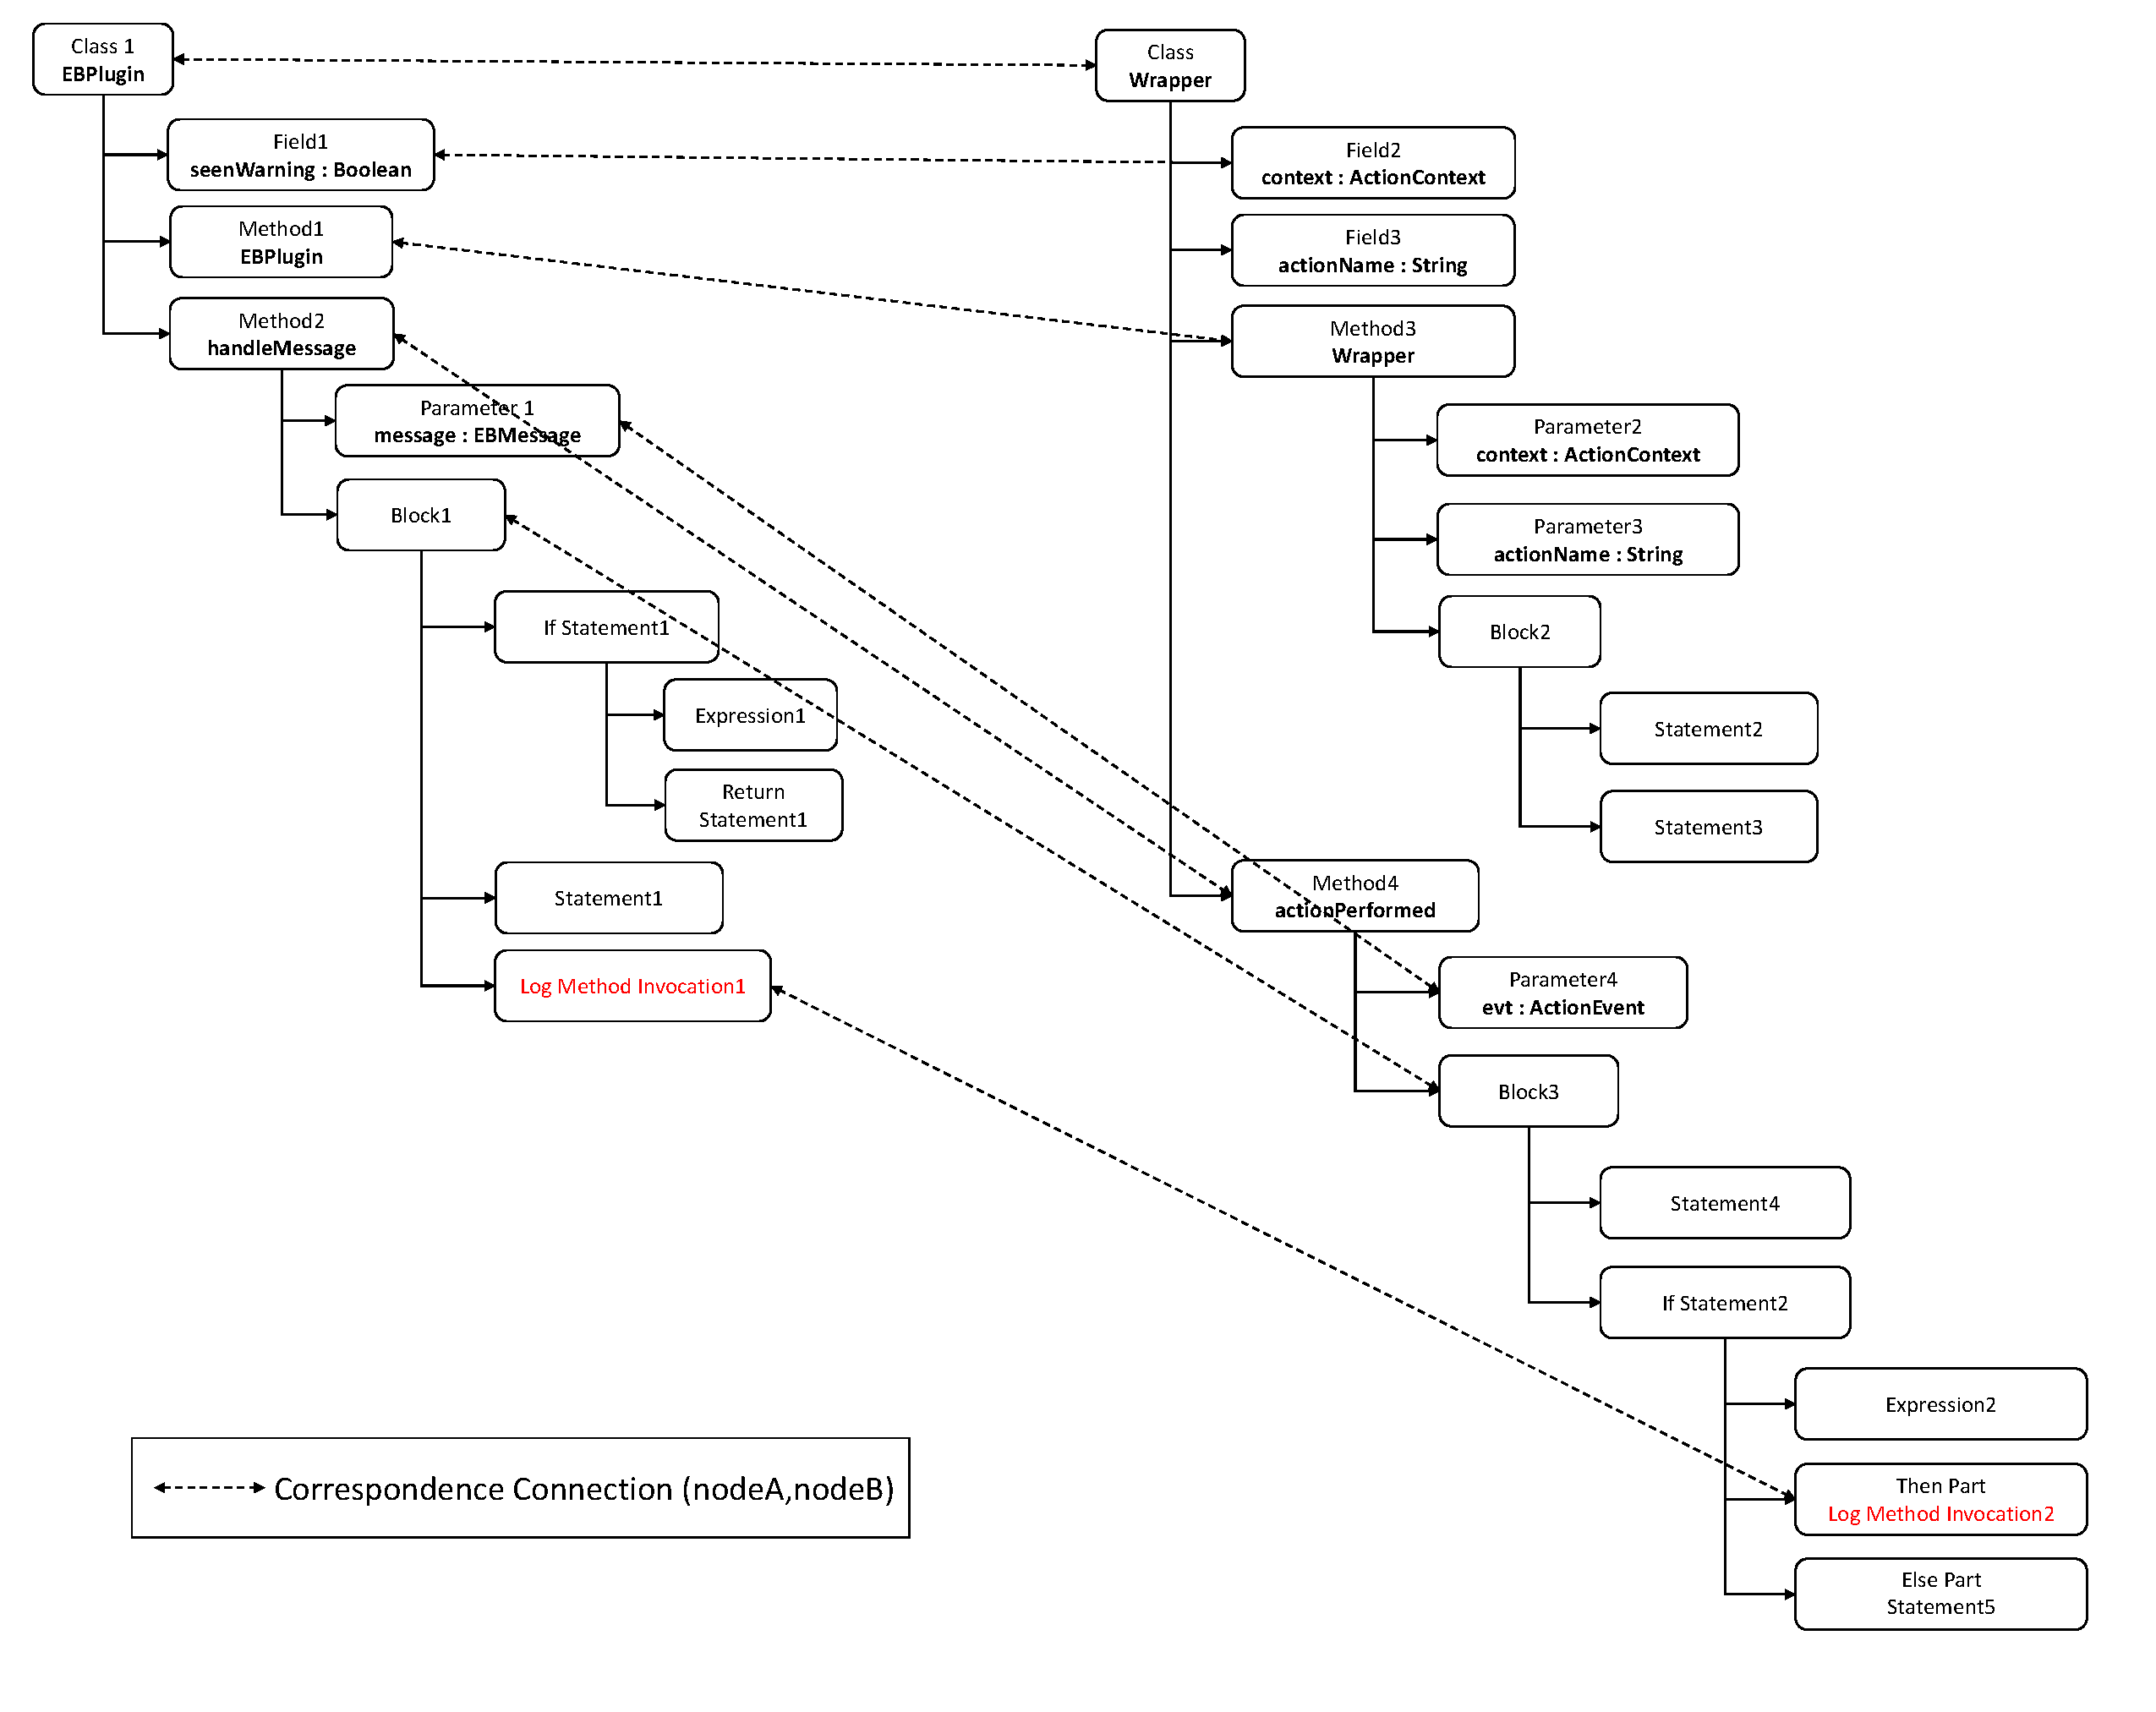
\includegraphics [width = \textwidth]{Drawing4/FinalCorr.pdf}
  \caption{Simple AUAST structures constructed from the ASTs in Figure~\ref{fig:meth-ast-1}. Links between AUAST nodes indicate structural correspondences selected as the best fit}
  \label{fig:AUASTs}
\end{figure}


\section{Computing Similarity} \label{meth-similarity}
Similarity computation is particularly important for the clustering phase that relies on accurate estimation of distance between logged Java classes. The notion of similarity can differ depending on the given context. That is, similarity between certain features could be highly important for a particular application, while it is not for the other one. The utility of a similarity function can be determined based on how good it enables us to produce accurate results for a particular task. In this study, a similarity measure is needed to classify Java classes that use logging calls based on structural similarity between them. The structural similarity of two AUASTs can be defined as the number of identical simple structural property values over total number of simple structural property values of the anti-unifier.

\begin{algorithm}
  \caption{\func{Compute-Matches}(\vars{auastA}, \vars{auastB}), determines the matches between two AUASTs via a recursive traversal of structural properties}
  \label{computeMatches}
  \begin{algorithmic}[1]
  \ComputeMatch
  	\If {$\vars{auastB} \neq \cons{NULL}$}
  	   \State{$ \func{Determine-Best-Correspondence}(\vars{auastA}, \vars{auastB})$}
  	   \EndIf
         \State $\vars{matches} \gets 0$
       \For {$\vars{property} \in \vars{properties}[\vars{ant-unifier}]$}
	\State $\vars{valueA} \gets \vars{value}[\vars{property}]$
	\State $\vars{valueB} \gets \vars{value}[\func{getCorrespondence}(valueA)]$
       	\If {$\vars{property}$  \Instanceof $\cons{SimpleProperty}$ \ori $\vars{property}$  \Instanceof $\cons{SimpleVariableProperty}$}
 \State $\vars{matches} \gets  \vars{matches} + \func{Jigsaw-Matches}(\vars{valueA}, \vars{valueB})$ 	    
	    
 		\ElsIf {$\vars{property}$ \Instanceof $\cons{ChildProperty}$ \ori $\vars{property}$  \Instanceof $\cons{ChildVariableProperty}$}		
	          \State $\vars{matches} \gets  \vars{matches} +\func{Compute-Matches}(\vars{valueA,valueB})$		
	    \ElsIf {$\vars{property}$ \Instanceof $\cons{ChildListProperty}$}
	\For {$\vars{nodeA} \in \vars{valueA}$}	  
		\State $\vars{nodeB} \gets \func{getCorrespondence}(\vars{nodeA})$    
	 \State $\vars{matches} \gets  \vars{matches} + \func{Compute-Matches}(\vars{nodeA}, \vars{nodeB})$
	  \EndFor 	
	   \EndIf
       \EndFor 	
	\Return $\vars{matches}$
  \end{algorithmic}
\end{algorithm}


The number of matches between \vars{auastA} and \vars{auastB} is computed via the \textsc{Compute-Matches} algorithm through a recursive traversal of structural properties of the nodes. First, the best correspondences are selected using the \func{Determine-Best-Correspondence} algorithm. For simple and simple variable structural properties, the number of matches is computed re-using the Jigsaw similarity function that computes the number of matches between the property values(Lines~8-9). For child and child variable structural properties, the number of matches is computed recursively for the child node and is propagated to the parent(Lines~10-11). For child list structural properties, the number of matches is computed for each child node recursively and is propagated to the parent node(Lines~12-17). All matches are summed up to compute total number of matches between the two AUASTs. Then the following equation is used to compute the structural similarity between \vars{auastA} and \vars{auastB}:

\begin{equation}\label{eq1}
\mbox{\vars{similarity}} = \frac{\mbox{2*\vars{matches}}}{\mid \mbox{\vars{auastA}} \mid + \mid \mbox{\vars{auastB}} \mid}
\end{equation}

Where total number of simple values for \vars{auastA} and \vars{auastB} is computed via \func{Compute-Matches}(\vars{auastA}) and \func{Compute-Matches}(\vars{auastB}), respectively. The similarity function returns a value between 0 and 1 where indicate zero and total class matching, respectively.

%The recursion process terminates if a simple or a variable structural property is reached.

\section{Constructing the Anti-unifier} \label{meth-antiUnifier}
Once the best correspondences has been determined between AUAST nodes, we construct a new anti-unified AUAST by traversing AUAST structures recursively and anti-unifying the structural properties. The new anti-unified structure is a generalization of two original structure, called anti-unifier, where common structural properties are represented by copy, and differences in structural properties are represented by structural variables. The variables may be inserted in place of any node in AUAST including both subtrees and leaves and can be substituted with proper original substructures to gain back to original structures.

Anti-unification of two AUAST nodes is performed through anti-unification of their structural properties, via the \func{Anti-unify} algorithm. For each structural property of \vars{auastA} and \vars{auastB}, where there is no corresponding property in the other AUAST, a structural variable property is created through anti-unifying the structural property with the NIL structure via the \func{Anti-unify-Property} algorithm and added to properties of the anti-unifier (Lines~3-6 and Lines~13-17); if both nodes has the same property but with different property values, a structural variable property is created via the \func{Anti-unify-Property} algorithm and appended to the anti-unifier structural properties (Lines~7-8); otherwise, if the two nodes has the same exact structural property, a copy of one of them is added to the anti-unifier structural properties (Lines~10-11).


\begin{algorithm}
 \caption{Input into \func{Anti-unify}(\vars{auastA}, \vars{auastB}) are two AUAST nodes. This algorithm construct an anti-unified AUAST node through anti-unification of input node's structural properties.}
  \label{antiUnify}
  \begin{algorithmic}[1]
\AntiUnify
\State{$ \vars{anti-unifier} \gets \cons{Null}$}
\For {$\vars{propA} \in \vars{properties}[\vars{auastA}]$}
	\State{$ \vars{valueA} \gets \vars{value}[\vars{property}]$}
	\If {$ \func{contains}(\vars{auastB},\vars{propA})= \cons{NULL}$}
		\State{$\func{AddProperty}(\vars{anti-unifier}, \func{Anti-unify-Property}(\vars{propA},\cons{NIL}))$}
	\ElsIf{$ \vars{valueA} \neq \vars{value}[\func{contains}(\vars{auastB},\vars{propA})]$}
	\State{$\func{AddProperty}(\vars{anti-unifier}, \func{Anti-unify-Property}(\vars{propA},\func{contains}(\vars{auastB},\vars{propA}))$}
	\Else
     \State{$\func{AddProperty}(\vars{anti-unifier}, \vars{propA})$}
	\EndIf
\EndFor
\For {$\vars{propB} \in \vars{properties}[\vars{auastB}]$}
	\If {$ \func{contains}(\vars{auastA},\vars{propB})= \cons{NULL}$}
		\State{$\func{AddProperty}(\vars{anti-unifier}, \func{Anti-unify-Property}(\vars{propB},\cons{NIL}))$}
	
	\EndIf	
\EndFor
\Return $\vars{anti-unifier}$
\end{algorithmic}
\end{algorithm}

Anti-unification of structural properties \vars{propA} and \vars{propB} is performed via the \func{Anti-unify-Property} algorithm. If \vars{propA} is a simple property, a simple variable property is constructed referring to two simple values (Lines~2-3); If structural property is a child property, a child variable structure is constructed (Line~5); if structural property is a child list property, for each child of \vars{propA} and \vars{propB}, where there is no correspondence in the other AUAST, an anti-unified node is created through anti-unifying the child node with the NIL structure via \func{Anti-unify} algorithm and added to the value of the anti-unified child list property; otherwise, the child node is anti-unified with its best correspondence (Lines~6-18).


\begin{algorithm}
 \caption{\func{Anti-unify-Property}(\vars{propA}, \vars{propB}) takes two structural properties and creates an anti-unified structural property.}
  \label{antiUnify}
  \begin{algorithmic}[1]
\AntiUnifyProperty
\State{$ \vars{property} \gets \cons{Null}$}

\If {$\vars{propA}$  \Instanceof $\cons{SimpleProperty}$}
	      \State $\vars{property} \gets  \func{Create-Simple-Variable-Property}(\vars{propA},\vars{propB})$
 	 \ElsIf {$\vars{propA}$ \Instanceof $\cons{ChildProperty}$}
			\State $\vars{property} \gets  \func{Create-Child-Variable-Property}(\vars{propA},\vars{propB})$
			 \ElsIf {$\vars{propA}$ \Instanceof $\cons{ChildListProperty}$}
	
	\For {$\vars{child} \in \vars{value}[\vars{propA}]$}	
	  \If {$\vars{correspondence}[\vars{child}] \neq \cons{NULL}$} 	
	  \State $\func{append}(\vars{children},\func{Anti-unify}(\vars{child}, \vars{correspondence}[\vars{child}]))$
	   \Else 	
	    \State $\func{append}(\vars{children},\func{Anti-unify}(\vars{child}, \cons{NIL}))$
	    \EndIf
      \EndFor
      \For {$\vars{child} \in \vars{value}[\vars{propB}]$}	
	  \If {$\vars{correspondence}[\vars{child}] = \cons{NULL}$} 	          	
	    \State $\func{append}(\vars{children},\func{Anti-unify}(\vars{child}, \cons{NIL}))$
	    \EndIf
      \EndFor
		\State $ \vars{value}[\vars{property}] \gets\vars{children} $

    \EndIf
\Return $\vars{property}$
\end{algorithmic}
\end{algorithm}

For example, we supply \func{Anti-unify} algorithm with the log method invocation nodes from the AUASTs in Figure~\ref{fig:constructAUast}. \texttt{EXPRESSION} and \texttt{ARGUMENTS} are similar in both AUASTs thus a copy of them will be added to structural properties of the anti-unified AUAST (Line~10); however, the simple value of Name property is different in both structures thus a call to \func{Anti-unify-Property} on Line~8 will return a simple structural variable. Figure~\ref{fig:AUAUAST} shows the anti-unified AUAST, where the annotation \texttt{WARNING-or-ERROR} is used to represent the simple structural variable that must be substituted with either \texttt{WARNING} or \texttt{ERROR} simple value to gain back to each original AUAST structure. The structural representation of the anti-unified AUAST is \texttt{EXPRESSION[EXPRESSION[IDENTIFIER[\bold{Log}]], ARGUMENTS[QUALIFIER[IDENTI\\FIER[\bold{Log}]], NAME[IDENTIFIER[\bold{WARNING-or-ERROR}]]}.

\begin{figure} [H]
  \centering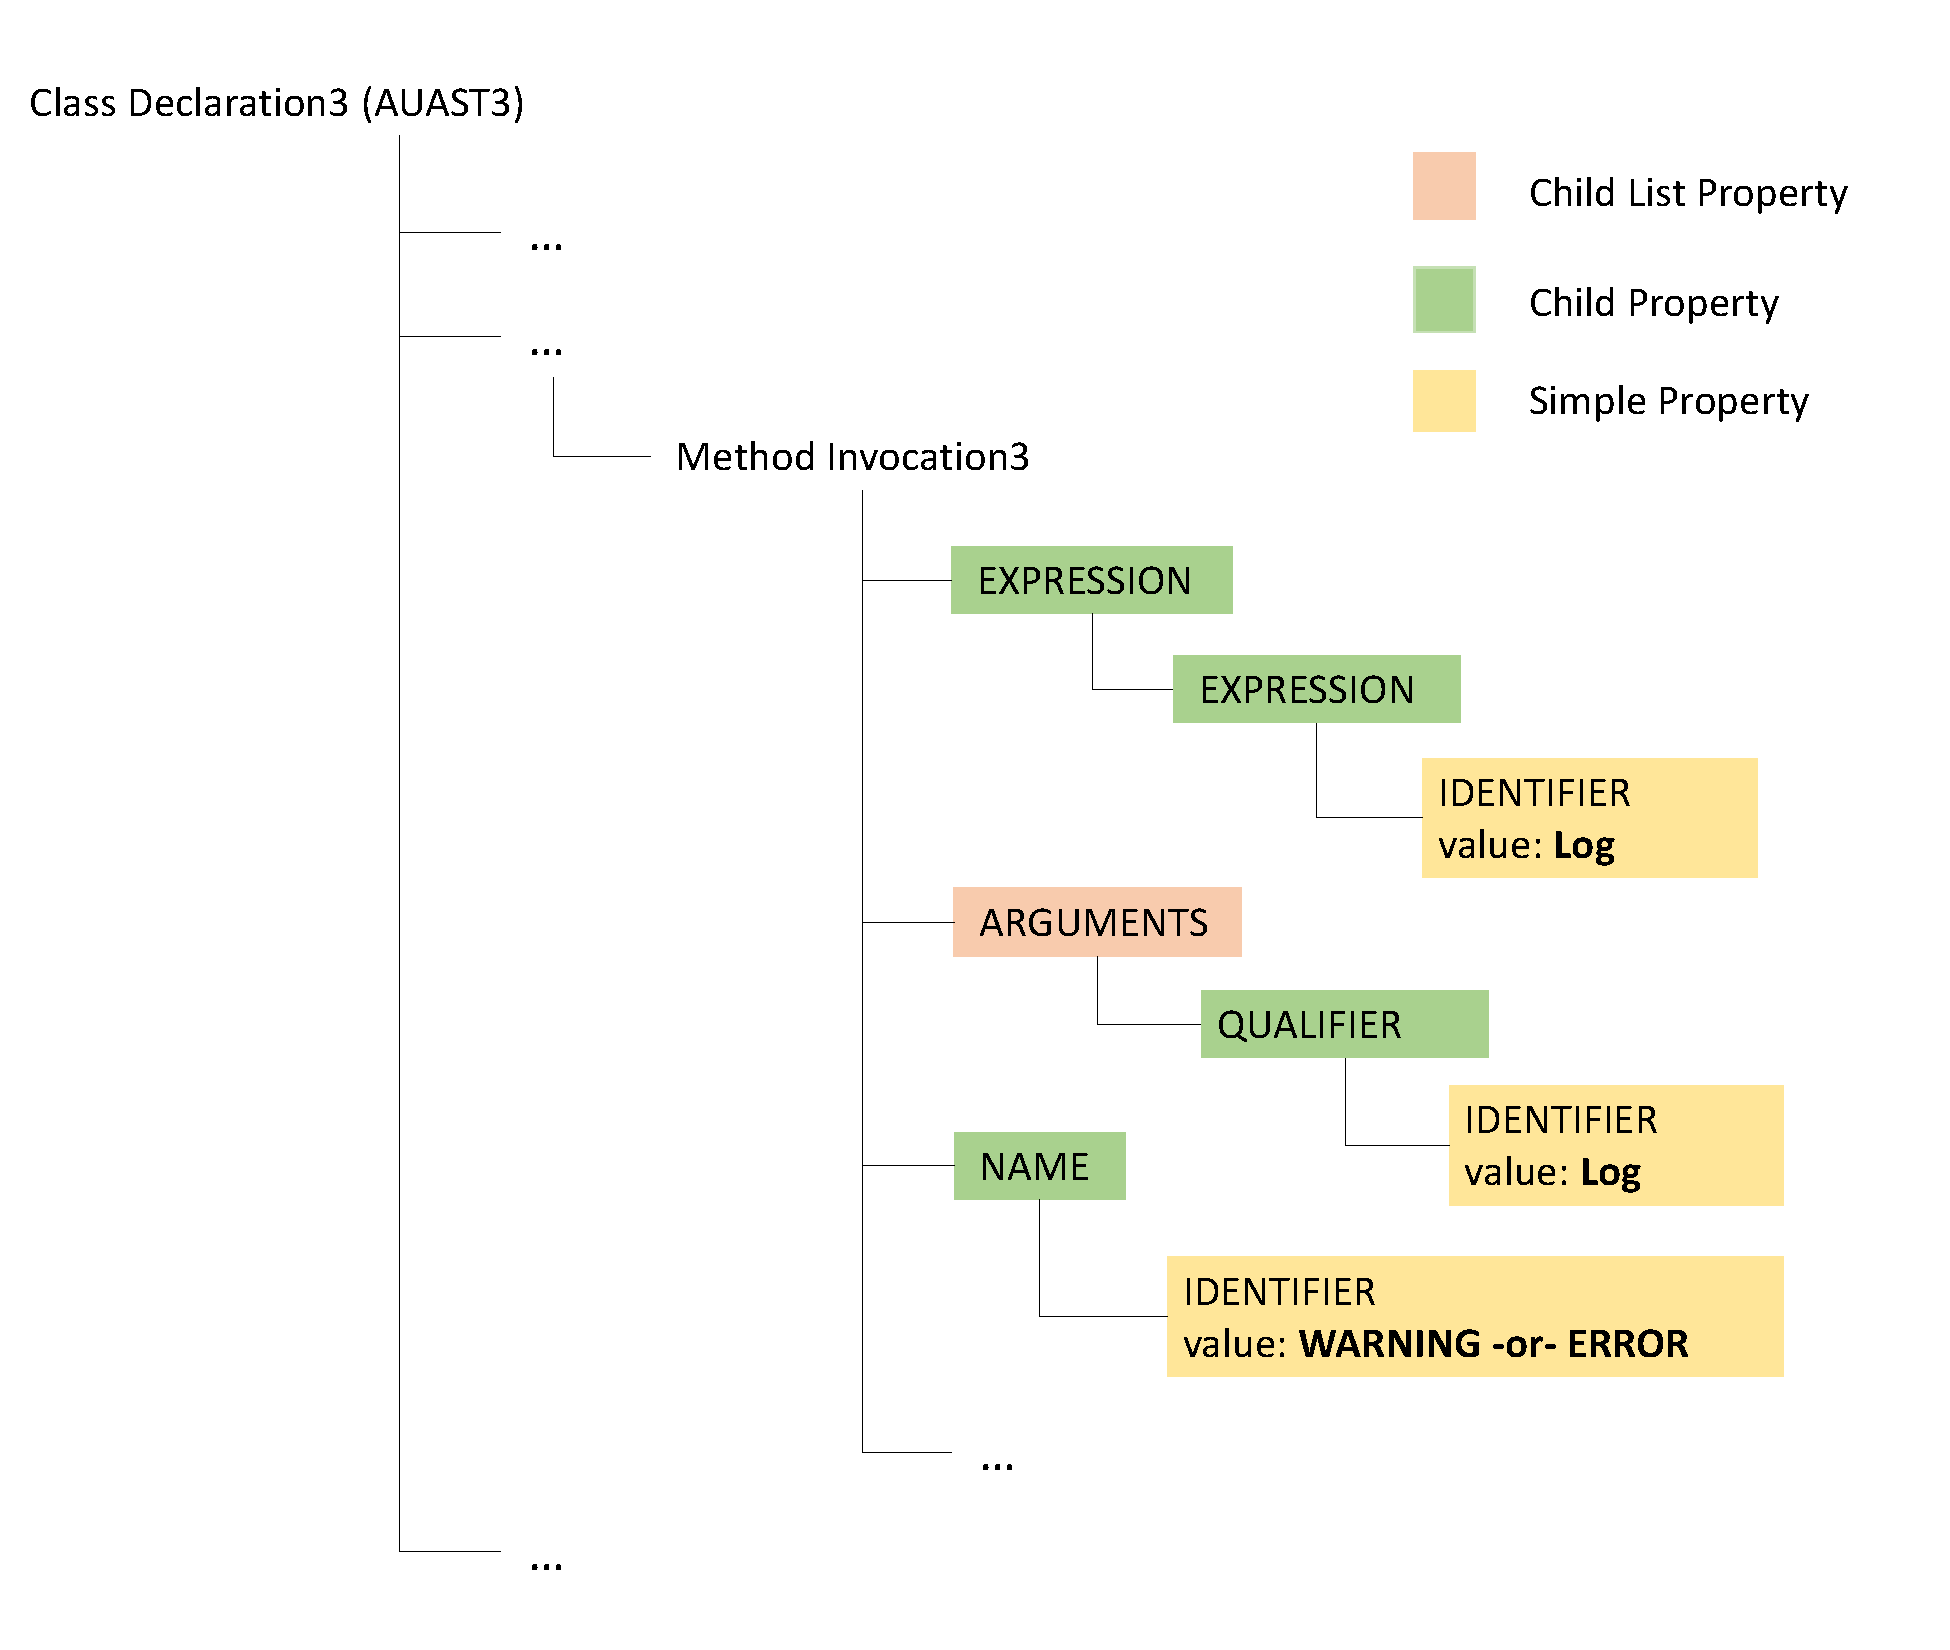
\includegraphics [width = 0.5\textwidth, height = 0.35\textheight]
  {Drawing4/structureAU.pdf}
  \caption{The anti-unifier (AUAST3) constructed from log Method Invocation AUAST nodes in Figure~\ref{fig:constructAUast} }
  \label{fig:AUAUAST}
\end{figure}

Figure~\ref{fig:meth-anti-unifier} shows a simple view of the anti-unified AUAST constructed from the two AUASTs in Figure~\ref{fig:AUASTs}, where ``$\vars{a}\langle\rangle\vars{b}$'' represents that the two subtrees \vars{a} and \vars{b} are anti-unified with each other in the anti-unifier and ``\vars{a}-or-\vars{b}'' represents a simple structural variable that must be substitutes with either \vars{a} or \vars{b} simple value to recover each original structure.


\begin{figure} [H]
  \centering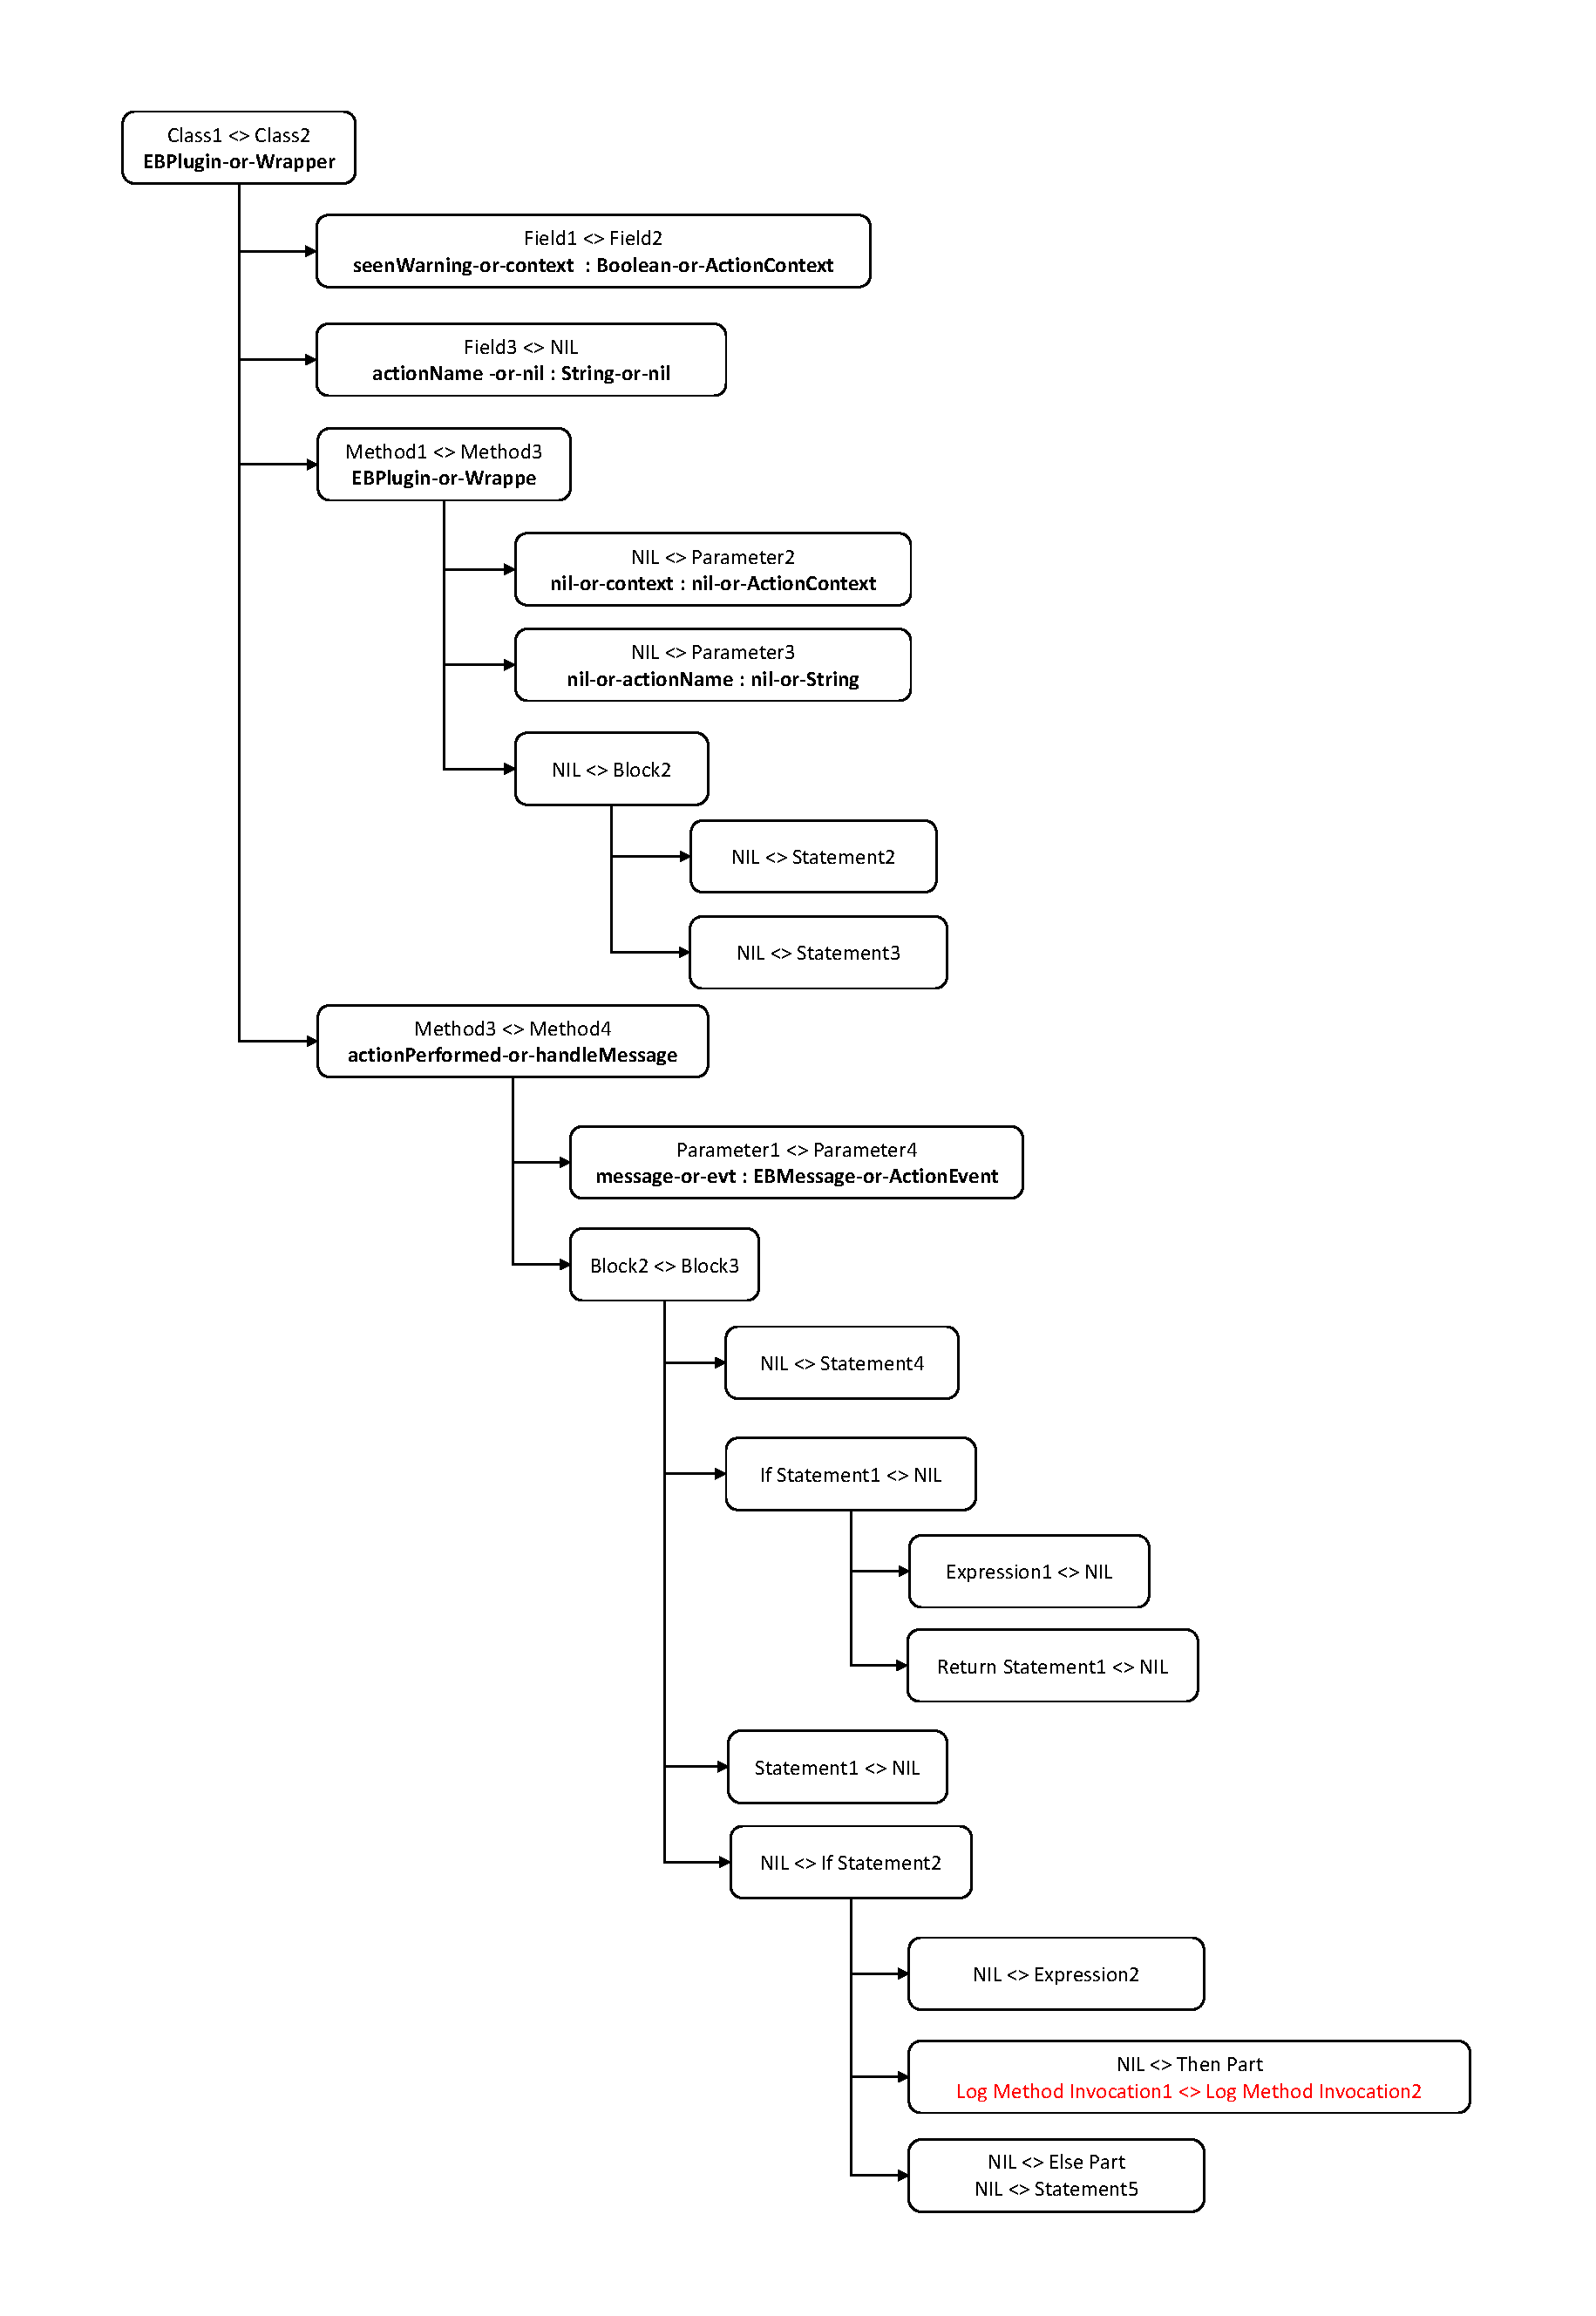
\includegraphics [width = 0.8\textwidth, height = 0.9\textheight]{Drawing4/Anti-unifier.pdf}
  \caption{Simple anti-unified AUAST structure of the two  AUASTs in Figure~\ref{fig:AUASTs}}
  \label{fig:meth-anti-unifier}
\end{figure}
\section{Multiple logging calls} \label{meth-multipleLogs}
\textbf{Problem:} There might be some cases that our approach is not able to anti-unify logging calls in two input seeds, when there is more than one logging call in a logged Java class. For example, consider the logged Java classes in Figures~\ref{multiple1} and~\ref{multiple2}. Figure~\ref{mast_1} shows the simple AUASTs for these examples and all potential correspondence connections between the AUAST nodes. Figure~\ref{m_ast2} shows the correspondence connections selected as the best match using our greedy algorithm. To anti-unify \vars{method1} with \vars{method3}, we should anti-unify their structural properties; thus, \vars{log1} should be anti-unified with \vars{log3} and  \vars{log4} should be anti-unified with \nothing since there is no corresponding logging call in the body of \vars{method 1}, while there is a corresponding logging call for \vars{log4} in the body of \vars{method2} (\vars{log2}).


\begin{figure}[H]
\def\baselinestretch{1}
\begin{lstlisting}
public class test1{
	public void method1(){
		...
		Log.log();
		...
	} 
	public void method2(){
		...
		Log.log();
		...
	} 
}
\end{lstlisting}
\caption{A Java class that utilizes multiple logging calls. This will be referred to as Example 1.\label{multiple1}}
\end{figure}



\begin{figure}[H]
\def\baselinestretch{1}
\begin{lstlisting}
public class test2{
	public void method3(){
		...
		Log.log();
		...
		Log.log();
	} 
}
\end{lstlisting}
\caption{A Java class that utilizes multiple logging calls. This will be referred to as Example 2.\label{multiple2}}
\end{figure}

\begin{figure} [H]
  \centering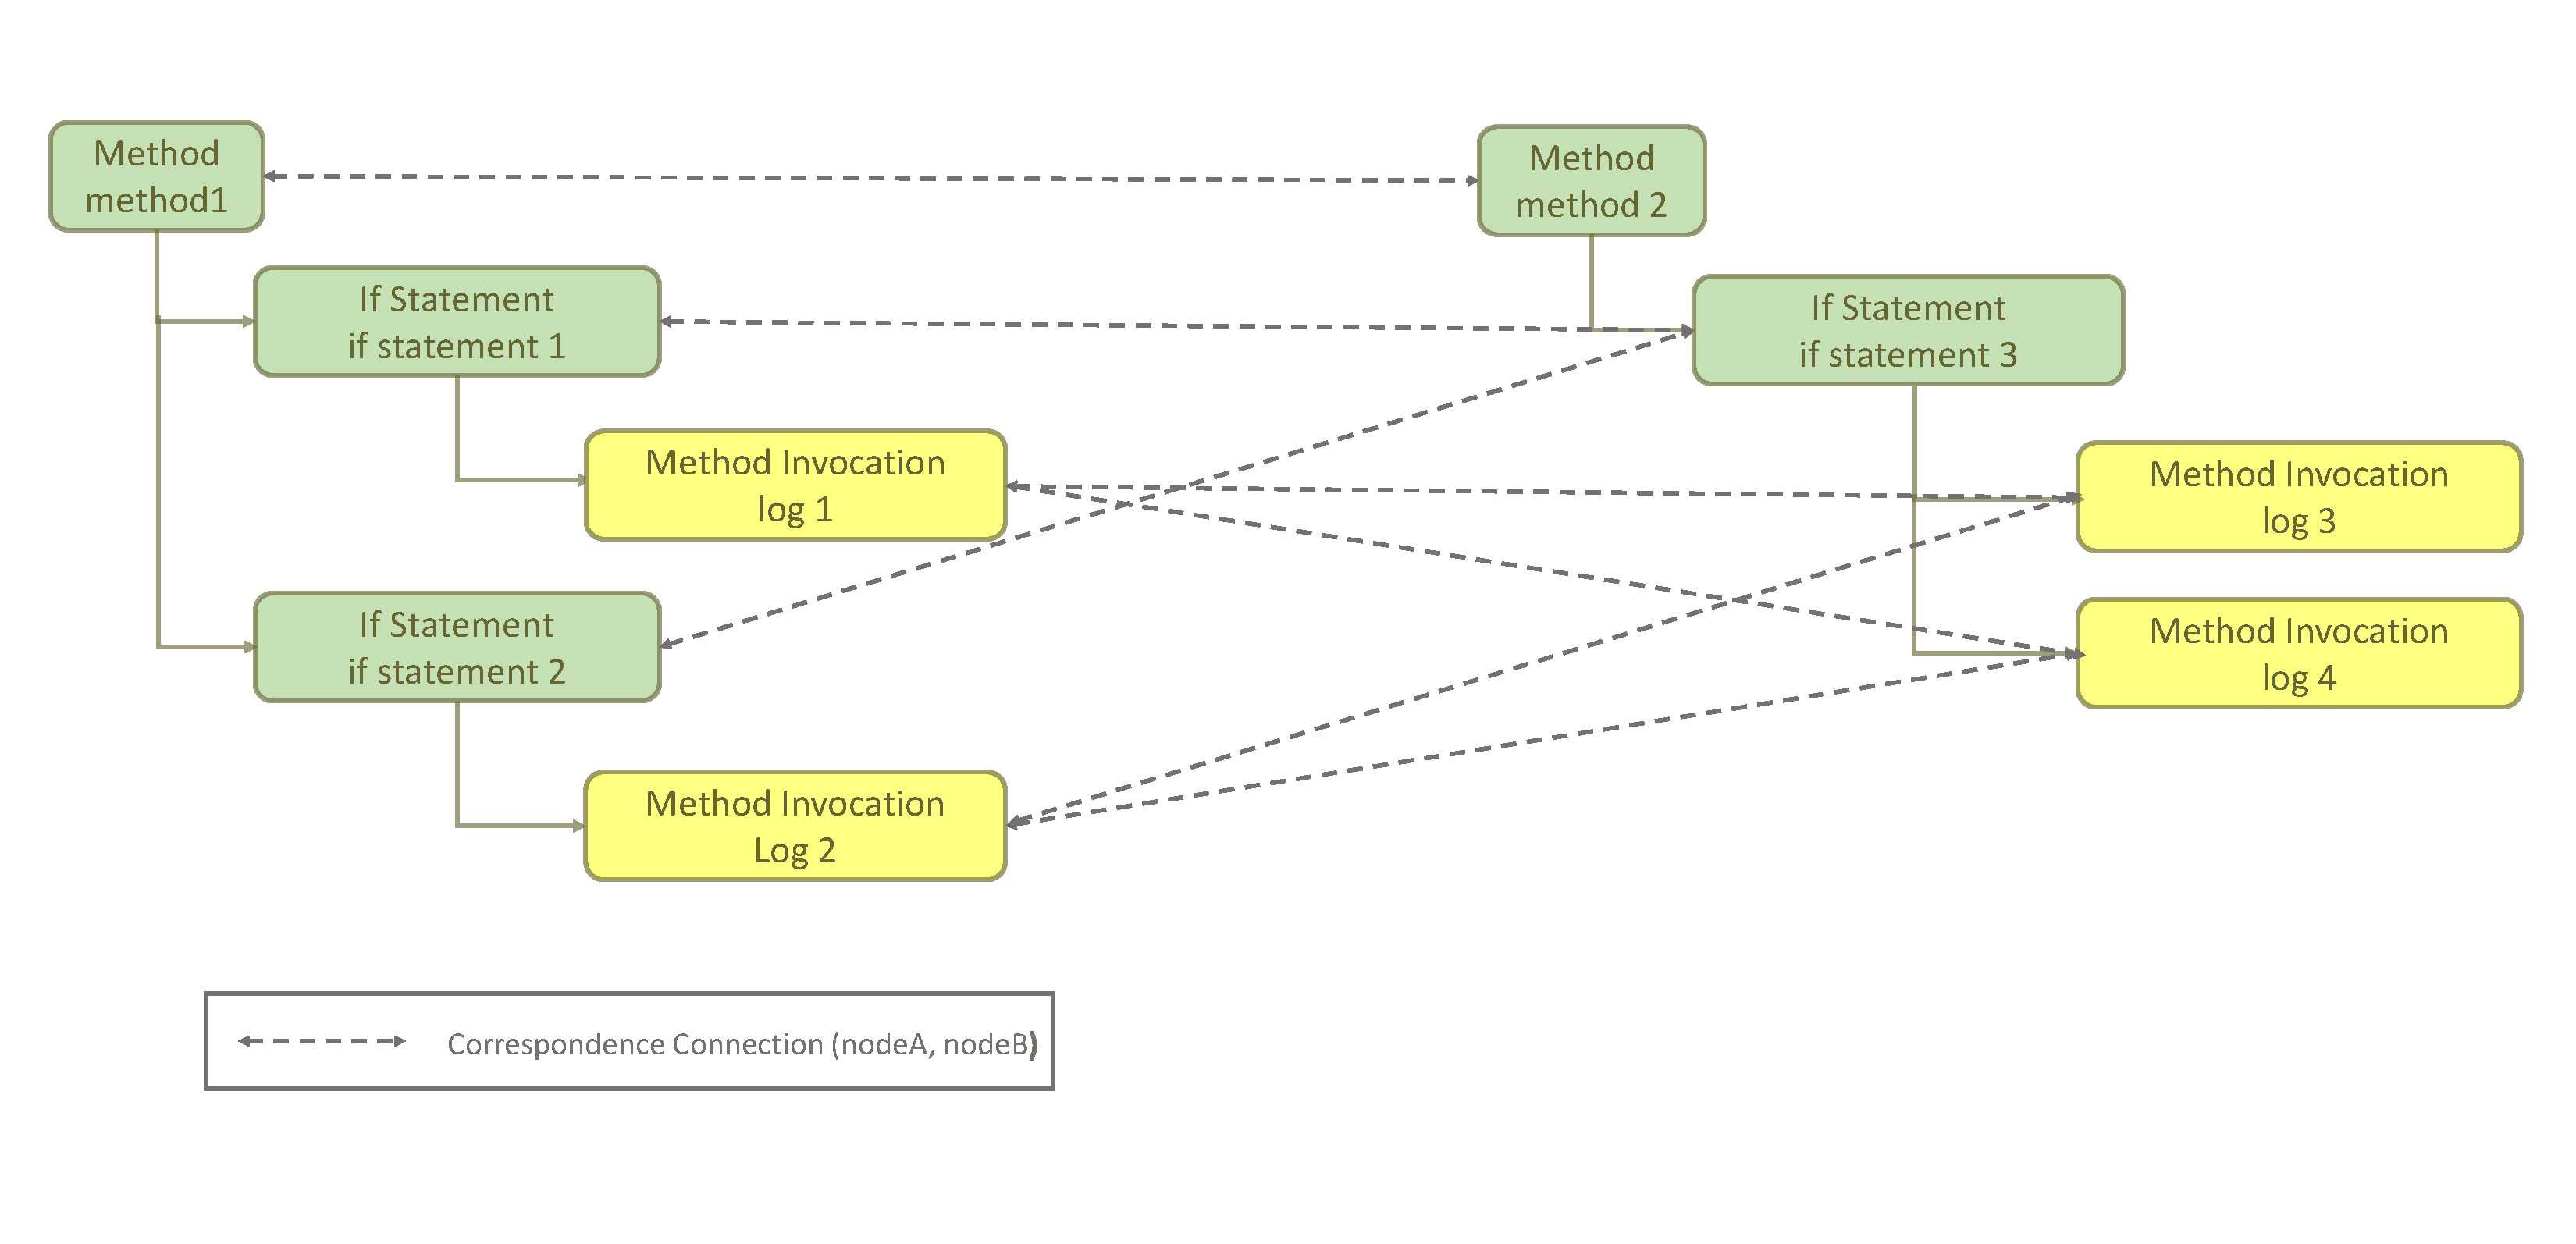
\includegraphics [width = \textwidth]{Drawing4/multipleLogging.pdf}
  \caption{Simple AUAST structure of examples in Figures~\ref{multiple1} and~\ref{multiple2}. Links between AUAST nodes indicate potential candidate structural correspondences detected by the Jigsaw framework.}
  \label{mast_1}
\end{figure}


\begin{figure} [H]
  \centering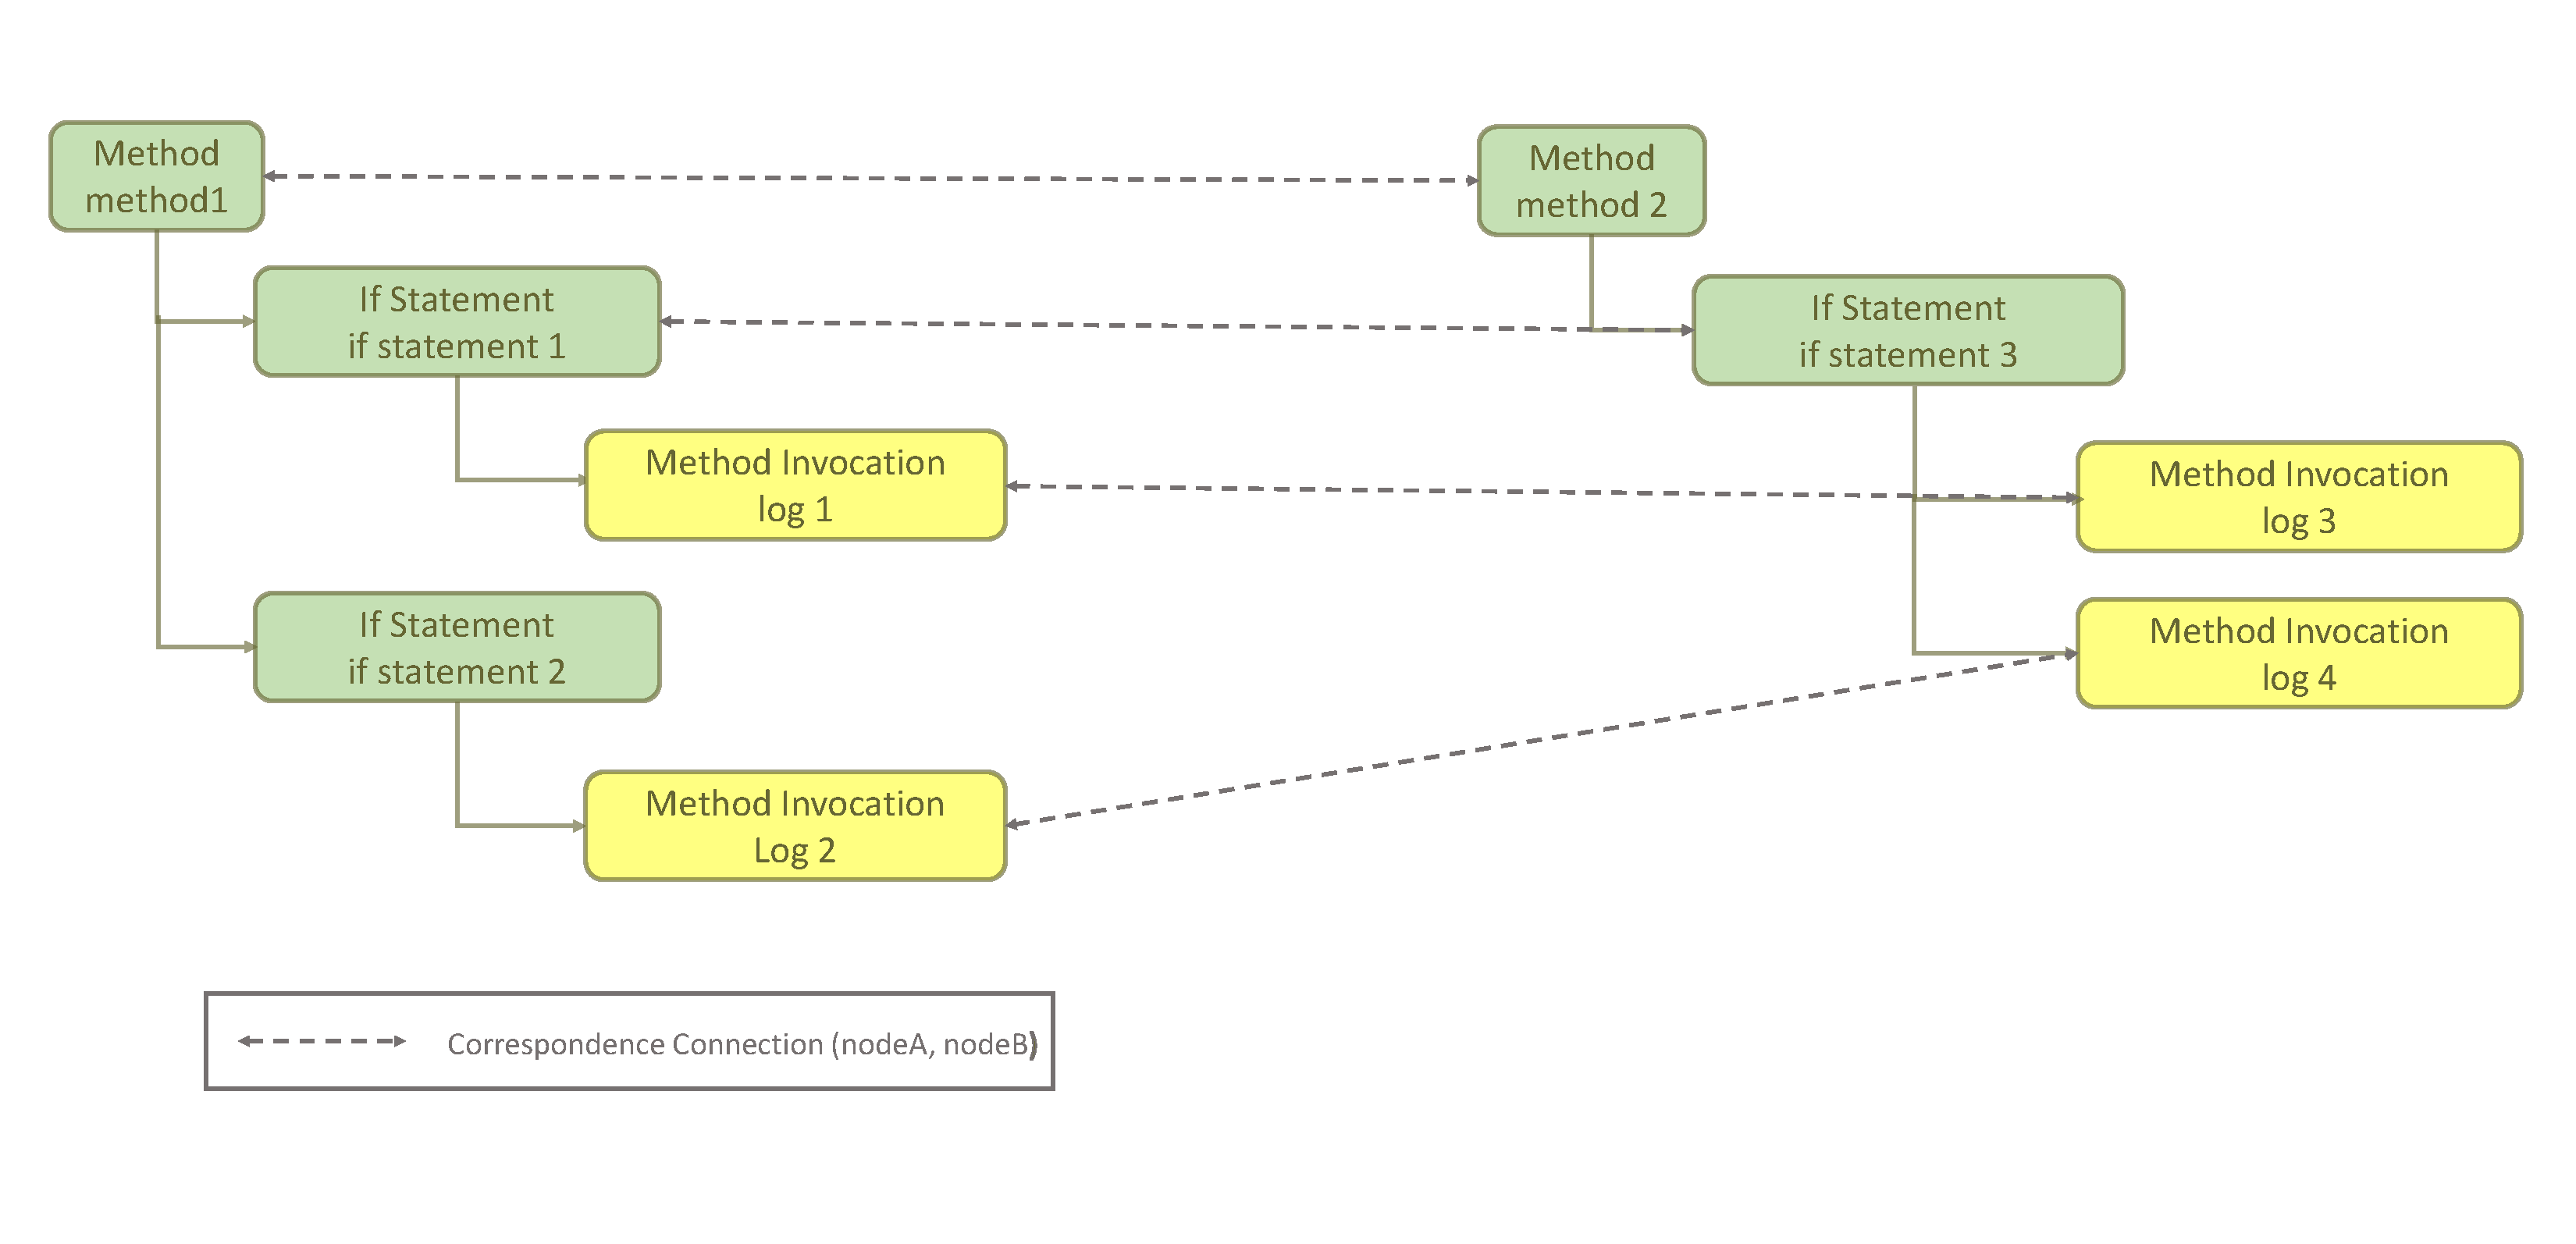
\includegraphics [width = \textwidth]{Drawing4/multipleLogging2.pdf}
  \caption{Simple AUAST structure of examples in Figures~\ref{multiple1} and~\ref{multiple2}. Links between AUAST nodes indicate structural correspondences selected as the best match using our greedy algorithm.}
  \label{m_ast2}
\end{figure}
 
\textbf{Suggested Solution:} We can split these cases into more than one case, where each logged Java class contains only one logging call. To do so, we need to create a copy of logged Java class for each logging call by maintaining the logging call and removing the other ones. For example, we need to create two copies for each logged Java class of Examples 1 and 2 as depicted in Figures~\ref{multiple1-one} and~\ref{multiple2-one}, respectively.
% thus constructing four possible anti-unifier for  possible combination and compute the similarity for each combination.   
%We can split this case into more than one case, each with one logging statement in every seed. That is, for each case all the other logging statements should be deleted from seeds.  For example, imagine we have AST 1 and AST 2. AST 1 contains three logging calls and AST 2 contains two logging calls. As explained, we split AST 1 into AST 1a, AST 1b, and AST 1c. Also, we split AST 2 into AST 2a and AST 2b. We can split this case into 6 possible cases and create an anti-unifier for each possible combination and then compute a measure of similarity for each case. The best match for each log statement can be selected based on anti-unifier with the highest similarity amongst the other options.


\begin{figure}[H]
\def\baselinestretch{1}
\begin{lstlisting}
public class test1{
	public void method1(){
		...
		Log.log();
		...
	} 
	public void method2(){
		...
		//removed
		...
	} 
}

public class test1{
	public void method1(){
		...
		//removed
		...
	} 
	public void method2(){
		...
		Log.log();
		...
	} 
}

\end{lstlisting}
\caption{Create multiple copies of Example 1 for each logging call.\label{multiple1-one}}
\end{figure}



\begin{figure}[H]
\def\baselinestretch{1}
\begin{lstlisting}
public class test2{
	public void method3(){
		...
		Log.log();
		...
		//removed
	} 
}

public class test2{
	public void method3(){
		...
		//removed
		...
		Log.log();
	} 
}

\end{lstlisting}
\caption{Create multiple copies of Example 2 for each logging call.\label{multiple2-one}}
\end{figure}



\section{Anti-unifying a set of AUASTs} \label{meth-clustering}
\begin{itemize} [leftmargin=.1in]
\item \textsc{Problem: } anti-unifying a set of AUASTs of LJCs
\item \textsc{Solution: }Developing a modified version of a hierarchical agglomerative clustering algorithm (illustrated in Figure~\ref{fig:overview2}) as described below: 
\begin{enumerate} [leftmargin=.3in]
\item Start with singleton clusters, where each cluster contains one AUAST 
\item Compute the similarity between clusters in a pairwise manner 
\item Find the closest clusters (a pair of clusters with maximum  similarity)
\item Merge the closest cluster pair and replace them with a new cluster containing anti-unifier of AUASTs of the two clusters 
\item Compute the similarity between the new cluster and all remaining clusters 
\end{enumerate}
\begin{itemize} [leftmargin=.3in]
\item Repeat Steps 3,4, and 5 until the similarity between closest clusters becomes below a predetermined threshold value
\item The similarity between a pair of clusters is defined as the similarity between their AUASTs 
\item Determine the similarity threshold value through informal experimentation 
\end{itemize}
\begin{figure} [H]
  \centering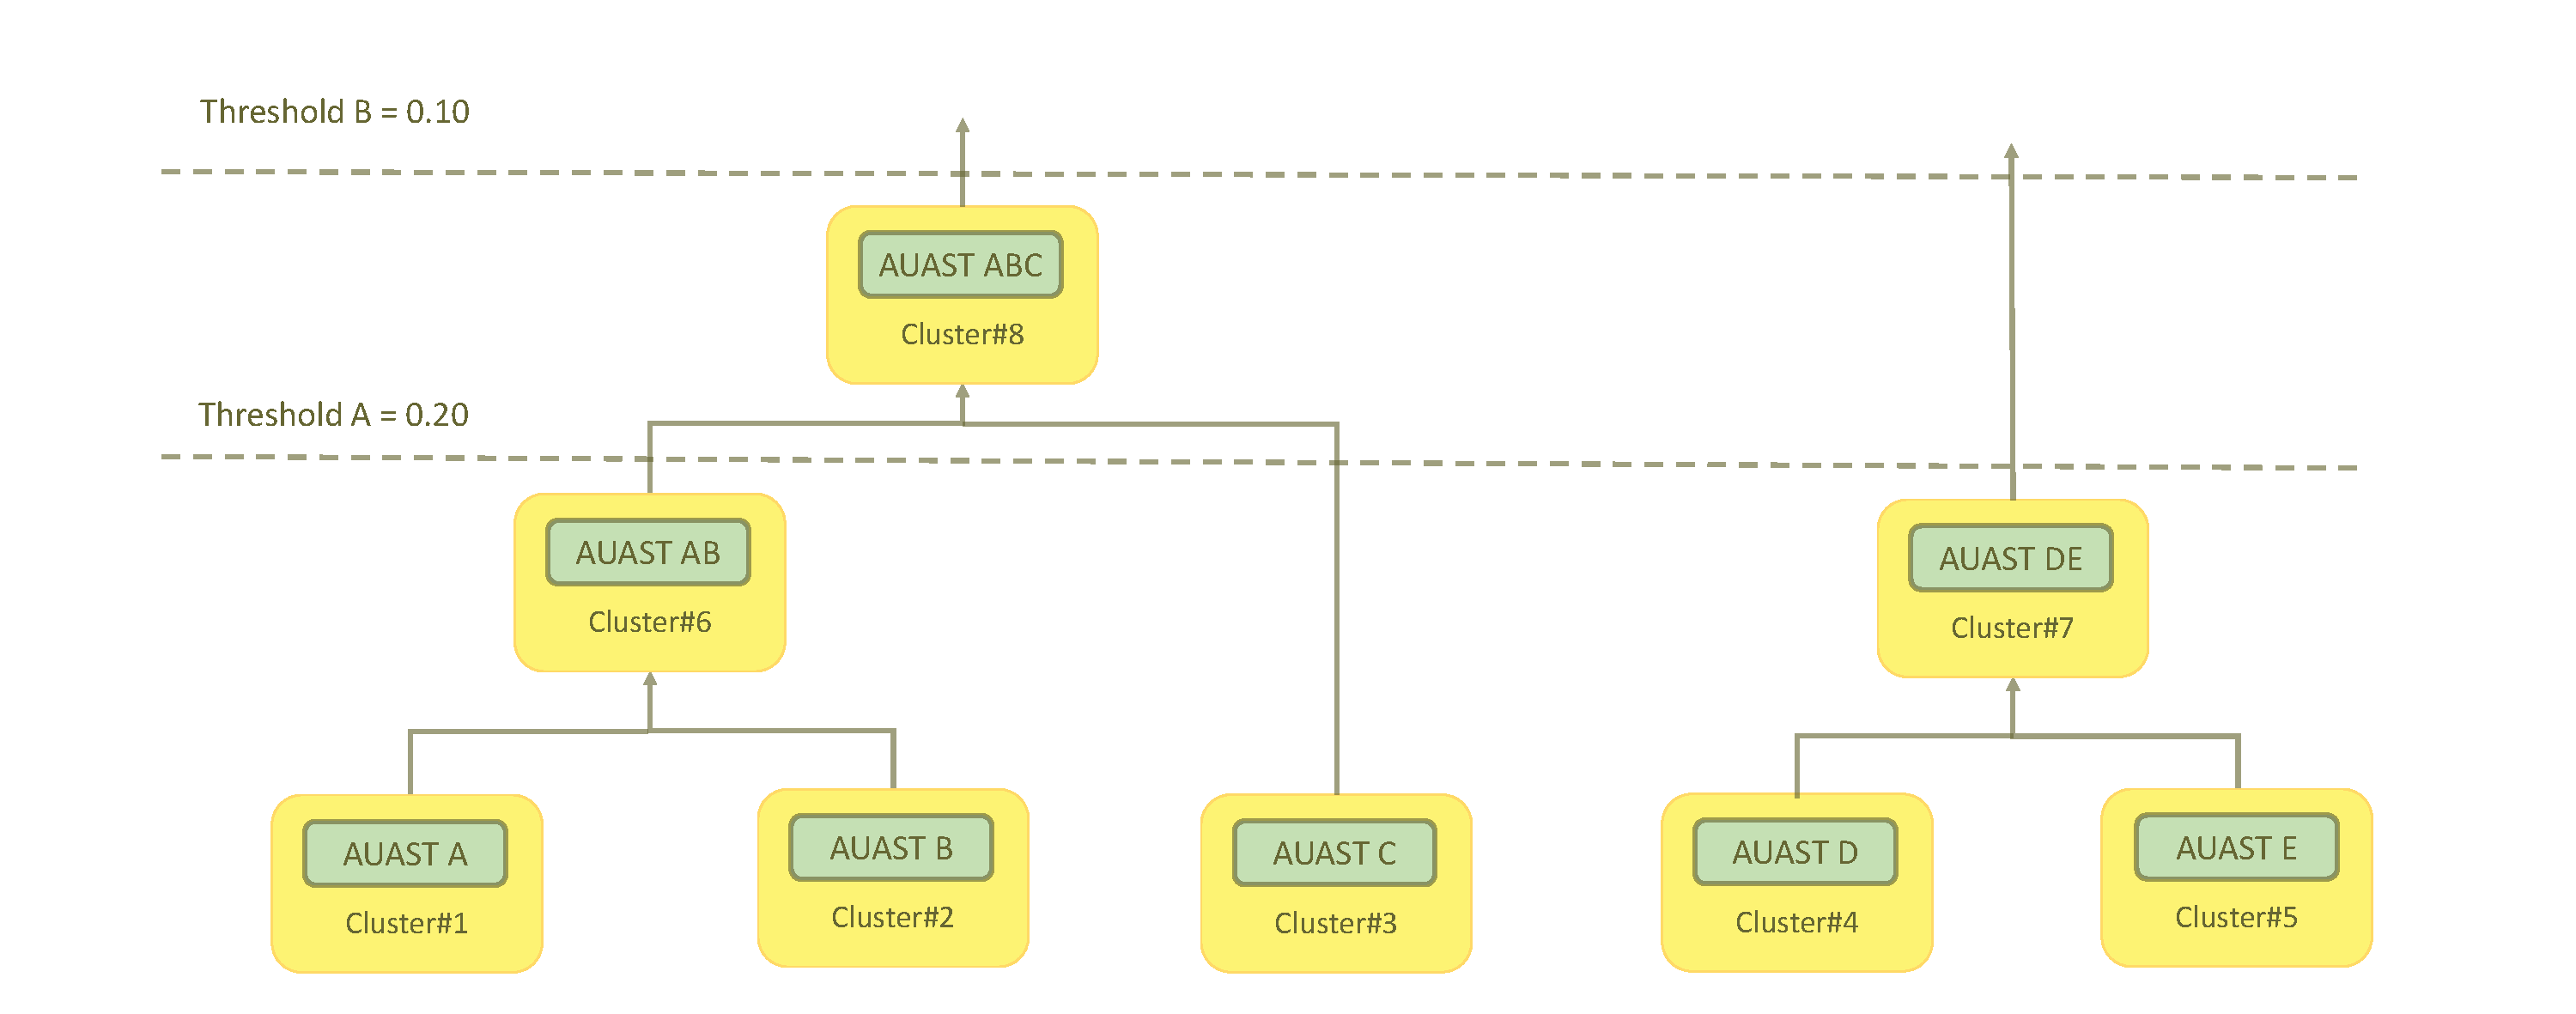
\includegraphics [width = \textwidth]{Drawing4/overview2.pdf}
  \caption{Anti-unification of 4 AUAST nodes using an agglomerative hierarchical clustering algorithm. The threshold value indicates the number of clusters we will come up with.}
  \label{fig:overview2}
\end{figure}
\end{itemize} 

%\section{Summary} \label{meth-summary}
%We have presented an approach to construct a generalization from ASTs of two logged Java classes with a special attention to log statements. This approach is implemented as an Eclipse plug-in tool, which given two logged Java classes utilizes the Jigsaw framework to identify potential correspondences between the two ASTs and greedily determines the best correspondence for each node with the highest Jigsaw similarity.  Moreover, some constraints have been applied on the selection of correspondences to deter anti-unifying log method invocation nodes with any other types of node. To anti-unify two structure, we make up a higher-order extended CAST structure, called AUAST, and construct the anti-unifier through the application of higher-order modulo theories over the extended structure. A measure of similarity has been developed to provide us with useful information for the clustering phase.